\documentclass[a4paper]{article}


\usepackage[T1]{fontenc}
\usepackage[utf8]{inputenc}
\usepackage{mathptmx}

%\usepackage{ngerman}	% Sprachanpassung Deutsch

\usepackage{graphicx}
\usepackage{geometry}
\geometry{a4paper, top=15mm}

\usepackage{subcaption}
\usepackage[shortlabels]{enumitem}
\usepackage{amssymb}
\usepackage{amsthm}
\usepackage{mathtools}
\usepackage{braket}
\usepackage{bbm}
\usepackage{graphicx}
\usepackage{float}
\usepackage{yhmath}
\usepackage{tikz}
\usepackage{algorithm}
\usepackage{algpseudocode}
\usetikzlibrary{patterns,decorations.pathmorphing,positioning}
\usetikzlibrary{calc,decorations.markings}

\newcommand{\eps}{\varepsilon}

\usepackage[backend=biber, sorting=none]{biblatex}
\addbibresource{uni.bib}

\usepackage[framemethod=TikZ]{mdframed}

\tikzstyle{titlered} =
    [draw=black, thick, fill=white,%
        text=black, rectangle,
        right, minimum height=.7cm]


\usepackage[colorlinks=true,naturalnames=true,plainpages=false,pdfpagelabels=true]{hyperref}
\usepackage[parfill]{parskip}
\usepackage{lipsum}


\usepackage{tcolorbox}
\tcbuselibrary{skins,breakable}

\pagestyle{myheadings}

\markright{Popović\hfill Tensor Methods \hfill}


\title{University of Vienna\\ Faculty of Mathematics\\
\vspace{1cm}TENSOR METHODS FOR DATA SCIENCE AND SCIENTIFIC COMPUTING
}
\author{Milutin Popovic}

\begin{document}
\maketitle
\tableofcontents
\section{Assignment 4}
\subsection{HOSVD Algorithm}
The HOSVD algorithm is used to compute the Tucker approximation of a given tensor $A \in \mathbb{R}^{n_1
\times \cdots \times n_d}$ with given ranks $r_1, \dots, r_d\ \in \mathbb{N}$ ($d
\in \mathbb{N}$ and $n_1, \dots, n_d\ \in \mathbb{N}$. Additionally we would
like to compute and save
\begin{itemize}
    \item  the Forbenius norms of the error produced at each step of the
            algorithm $\frac{\| A - \hat{A}_k\|_F}{\|A\|_F}$ and the vectors of
    \item the vector of singular values directly approximated by the
        algorithm
\end{itemize}
The Tucker decomposition for $A$, with the ranks above is the following
\begin{align}
    A_{i_1,\cdots,i_d} = \sum_{\alpha_1=1}^{r_1} \cdot
    \sum_{\alpha_d=1}^{r_d} (U_1)_{i_1,\alpha_1} \cdots (U_d)_{i_d,\alpha_d}
    S_{\alpha_1, \dots, \alpha_d},
\end{align}
where $U_k \in \mathbb{R}^{n_k \times r_k}$ for all $k \in \{1, \cdots, d\}$
and $S \in \mathbb{R}^{r_1 \times \cdots \times r_d}$ is called the
Tucker-core.

The HOSVD algorithm with the additional requirements for the Tucker
decomposition of $A$ is the following
\begin{algorithm}[H]
  \caption{HOSVD algorithm}\label{alg: hosvd}
\begin{algorithmic}
    \State $\hat{S}_0 \gets A$
    \State $A_0 \gets A$
    \For{$k = 1, \dots, d$}
        \State $(B_k)_{\alpha_1\cdots\alpha_{k-1}\cdot i_{k+1} \cdots
        i_d,i_k} \gets (\hat{S}_{k-1})_{\alpha_1, \dots, \alpha_{k-1}, i_k,
        \dots, i_d}$ \Comment{permute then reshape}

        \State $\hat{B}_k \gets \hat{U}_k \hat{\Sigma}_k \hat{V}_k^*$
        \Comment{rank $r_k$ T-SVD for $B_k$}

        \State $(\hat{S}_k)_{\alpha_{1}, \dots, \alpha_{k}, i_{k+1},\dots,i_d
        } \gets (B_k \hat{V}_k)_{\alpha_{1}, \dots, \alpha_{k-1}, i_{k+1}, \dots,
        i_d, \alpha_k}$ \Comment{reshape then permute}

        \State $(A_k)_{i_1,\cdots,i_d} \gets \sum_{\alpha_1=1}^{r_1} \cdot
        \sum_{\alpha_k=1}^{r_k} (\hat{V}_1)_{i_1,\alpha_1} \cdots (\hat{V}_k)_{i_d,\alpha_d}
        S_{\alpha_1, \dots, \alpha_{k}, i_{k+1}, \dots, i_d}$

        \State \text{save} $\frac{\| A - \hat{A}_k\|_F}{\|A\|_F}$
        \State \text{save} $\hat{V}_k$
        \State \text{save} $\hat{\Sigma}_k$
        \EndFor
\end{algorithmic}
\end{algorithm}
We note that at the $k-th$ step of the algorithm the shapes of the tensors
are
\begin{align}
    \hat{S}_{k-1} &\in \mathbb{R}^{r_1 \times \cdots \times r_{k-1} \times n_k
    \times \cdots n_d} \\
        \hat{V}_k &\in \mathbb{R}^{n_k \times r_k},\\
        \hat{B}_k &\in \mathbb{R}^{r_1\cdots r_{k-1}\cdot n_{k+1} \cdots n_d,
        \times n_k},\\
        \hat{\Sigma}_k &\in \mathbb{R}^{r_k \times 1}.
\end{align}
\subsection{Testing the HOSVD}
For the case $d=4$ we construct a quasirandom Tucker decomposition by drawing
the entries for $U_k \in \mathbb{R}^{n_k \times r_k}$ and $S \in \mathbb{R}^{r_1
\times \cdots \times r_d}$ uniformly on $[-1, 1]$. The output of the errors in
the $k-th$ steps is in the figure bellow
\begin{figure}[H]
    \centering
    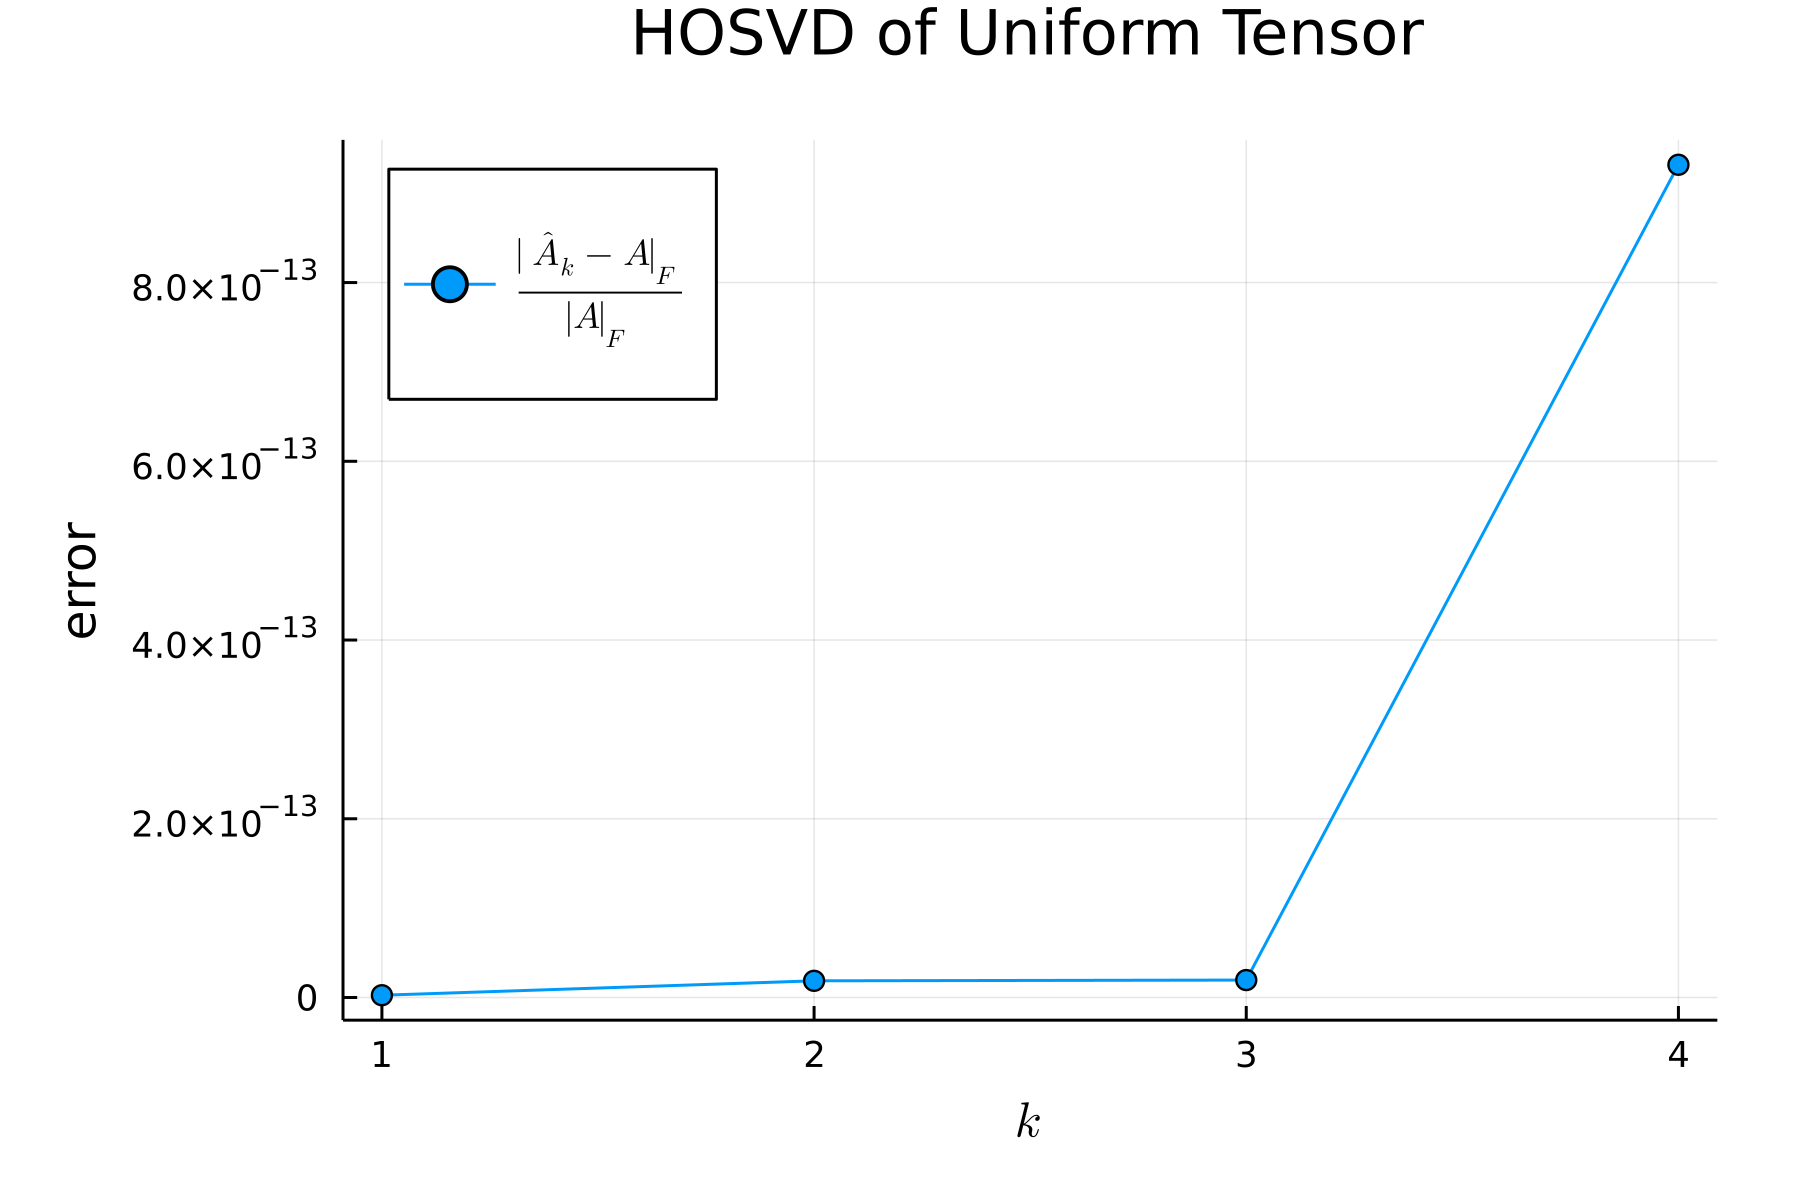
\includegraphics[width=\textwidth]{"./plots/hosvd-uniform-error.png"}
    \caption{Tucker approximation error on the $k-th$ step of a quasirandom
    Tensor}
\end{figure}
\subsection{Tucker approximation of function-related tensors \label{sec:
repeat}}
Consider two multivariable functions $f(x_1, \dots, x_d)$ and $g(x_1, \dots,
x_d)$, defined as
\begin{align}
    f(x_1, \dots, x_d) &= \left(1+\sum_{k=1}^d \frac{x^2_k}{8^{k-1}}
        \right)^{-1}\\
    g(x_1, \dots, x_d) &= \sqrt{\sum_{k=1}^d \frac{x_k^2}{8^{k-1}}} \cdot
    \left(1+\frac{1}{2}\cos\left(\sum_{k=1}^d \frac{4\pi x_k}{4^{k-1}}\right) \right)
\end{align}
for $x_1, \dots, x_d \in [-1, 1]$. Additionally we define a grid of points
\begin{align}
    t_i = 2 \frac{i-1}{n-1} -1 ,
\end{align}
for $i = 1, \dots, n$. With this we can construct a $d$ dimensional tensor of
size $n \times \cdots \times n$ by
\begin{align}
    b_{i_1, \cdots, i_d} = f(t_{i_1}, \dots, t_{i_d}),\\
    a_{i_1, \cdots, i_d} = g(t_{i_1}, \dots, t_{i_d}),
\end{align}
for all $i_1, \cdots, i_d \in \{1, \cdots, n\}$.

For $C = A$ and $C =B$.
For every $k \in \{1, \dots , d\}$, we compute the singular values of the $k-th$
Tucker unfolding matrix of C.
\begin{figure}[H]
    \centering
    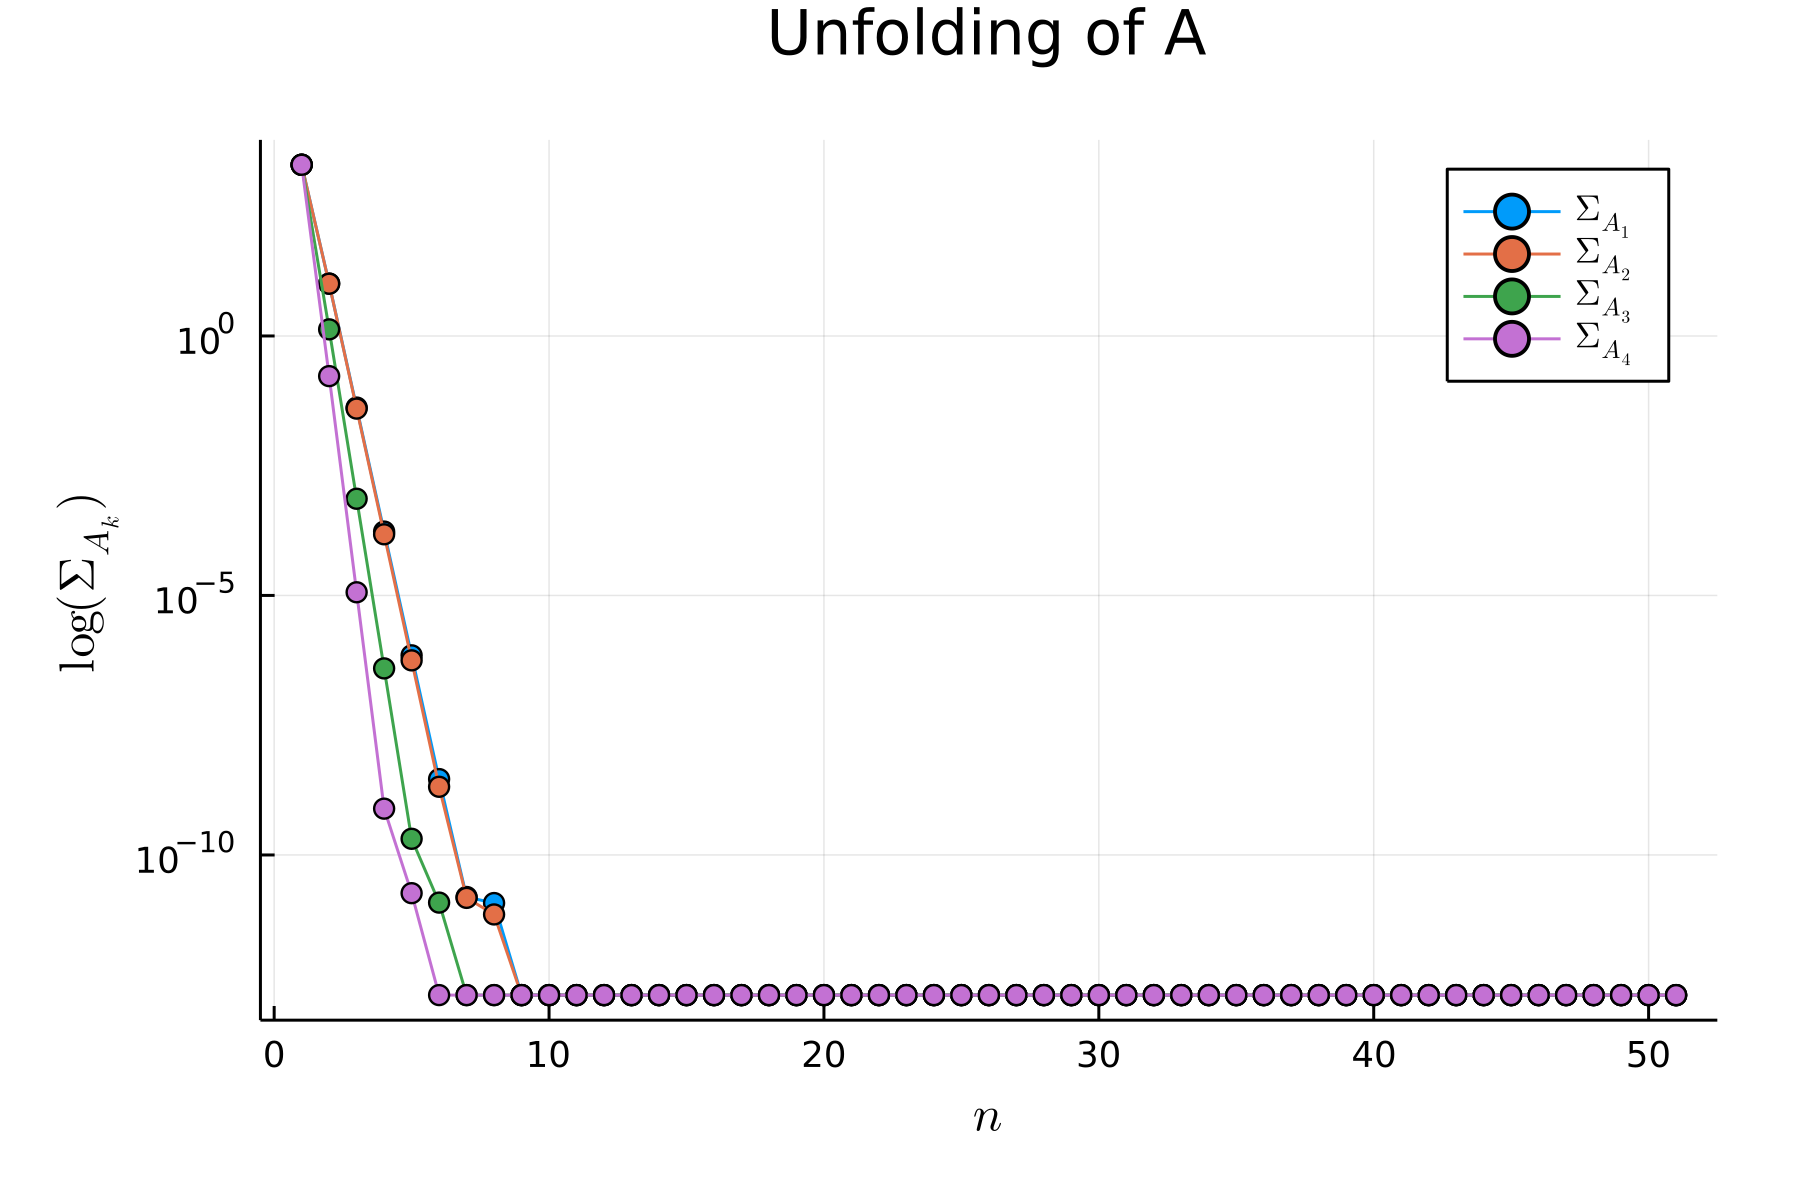
\includegraphics[width=0.49\textwidth]{./plots/singular-dec-A.png}
    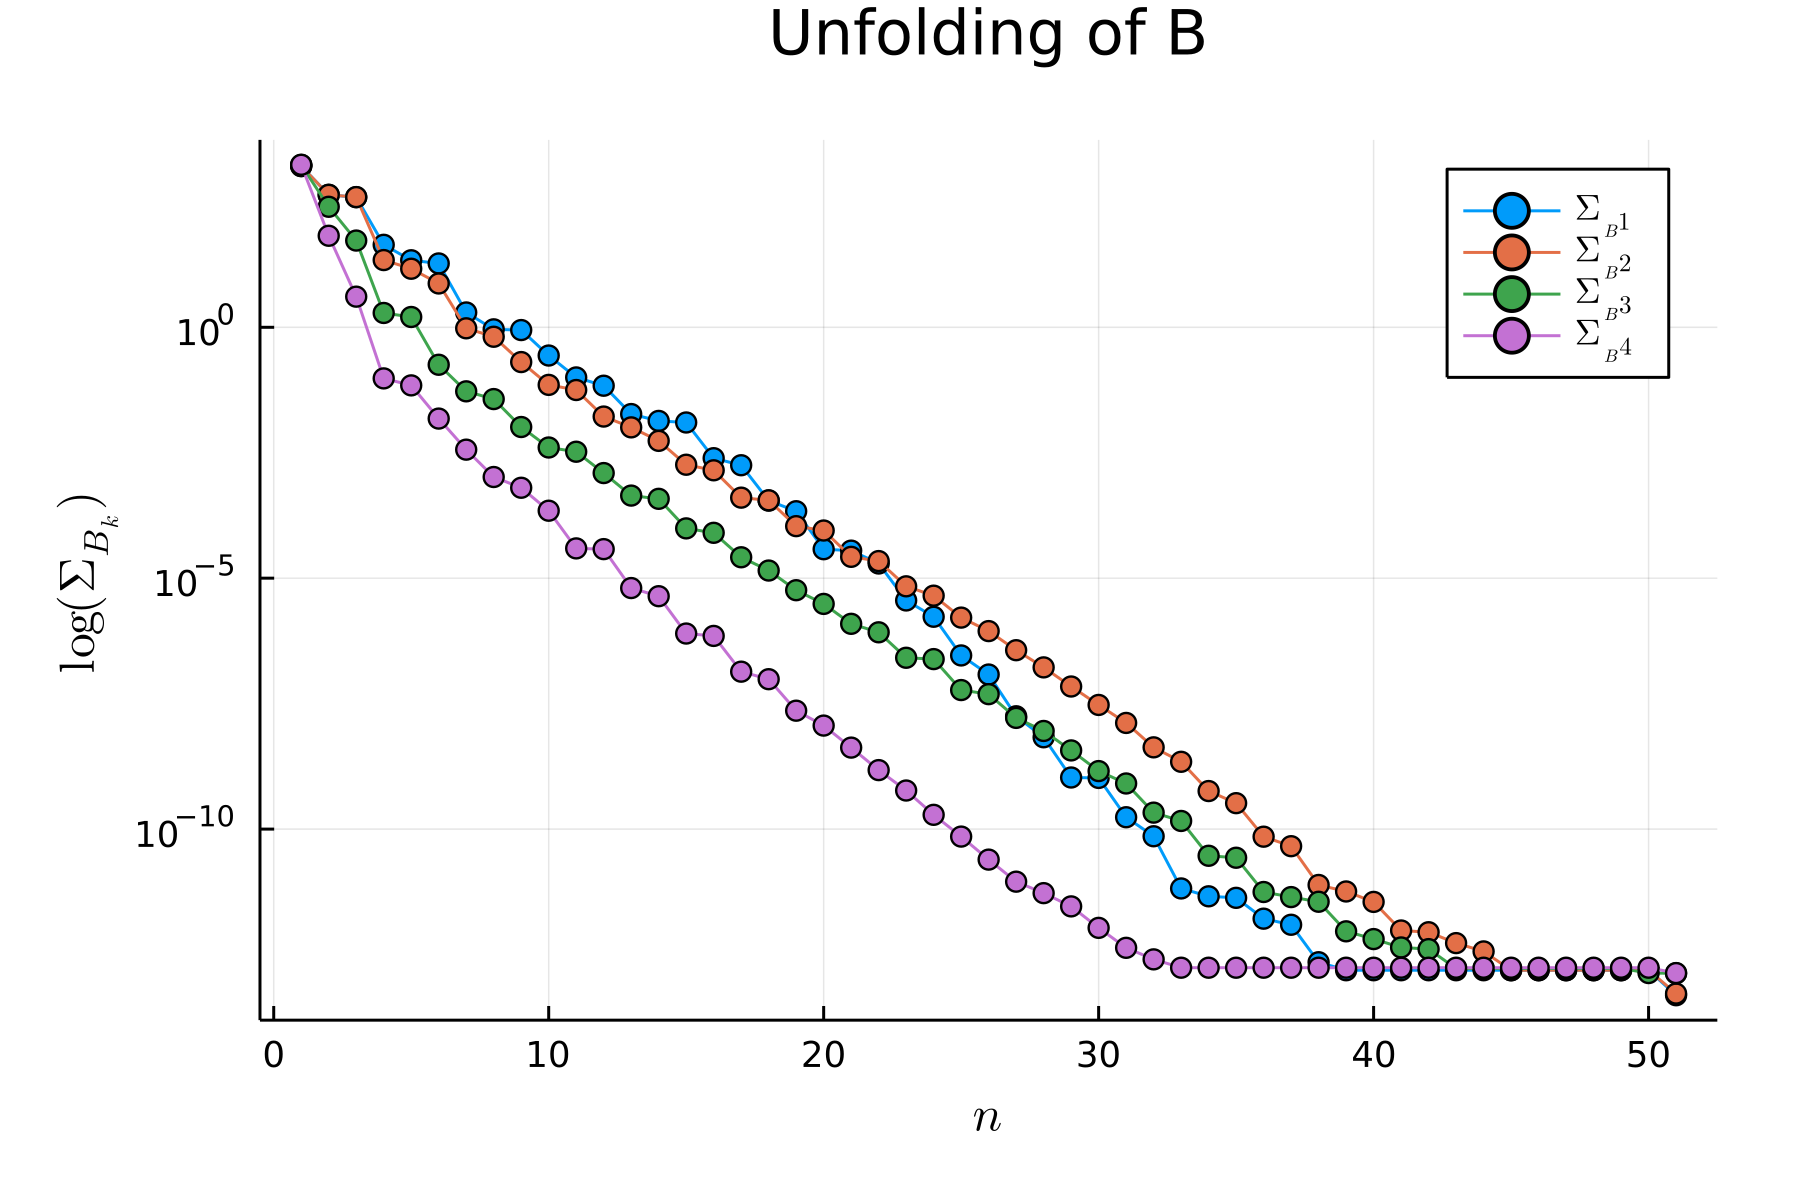
\includegraphics[width=0.49\textwidth]{./plots/singular-dec-B.png}
    \caption{Decrease of singular values of the $k-th$ Tucker unfolding of A,
    B produced by its SVD}
\end{figure}

For the accuracy Threshold $\eps_j = 10^{-j}$ with $j \in \{2, 4, \dots,
12\}$, for each $j$ and every $k$ we find the smallest $r_{jk}$ such that the
$k-th$ unfolding matrix can be approximated with ranks $r_{jk}$, where the
approximations relative error does not exceed $\eps_j$. Additionally we
compute the $\eps_{jk}$ error in the $k-th$ unfolding, which
should by the error analysis be bounded by $\eps_{jk} \leq \eps_{j}$ for all
$j$.
\begin{figure}[H]
    \centering
    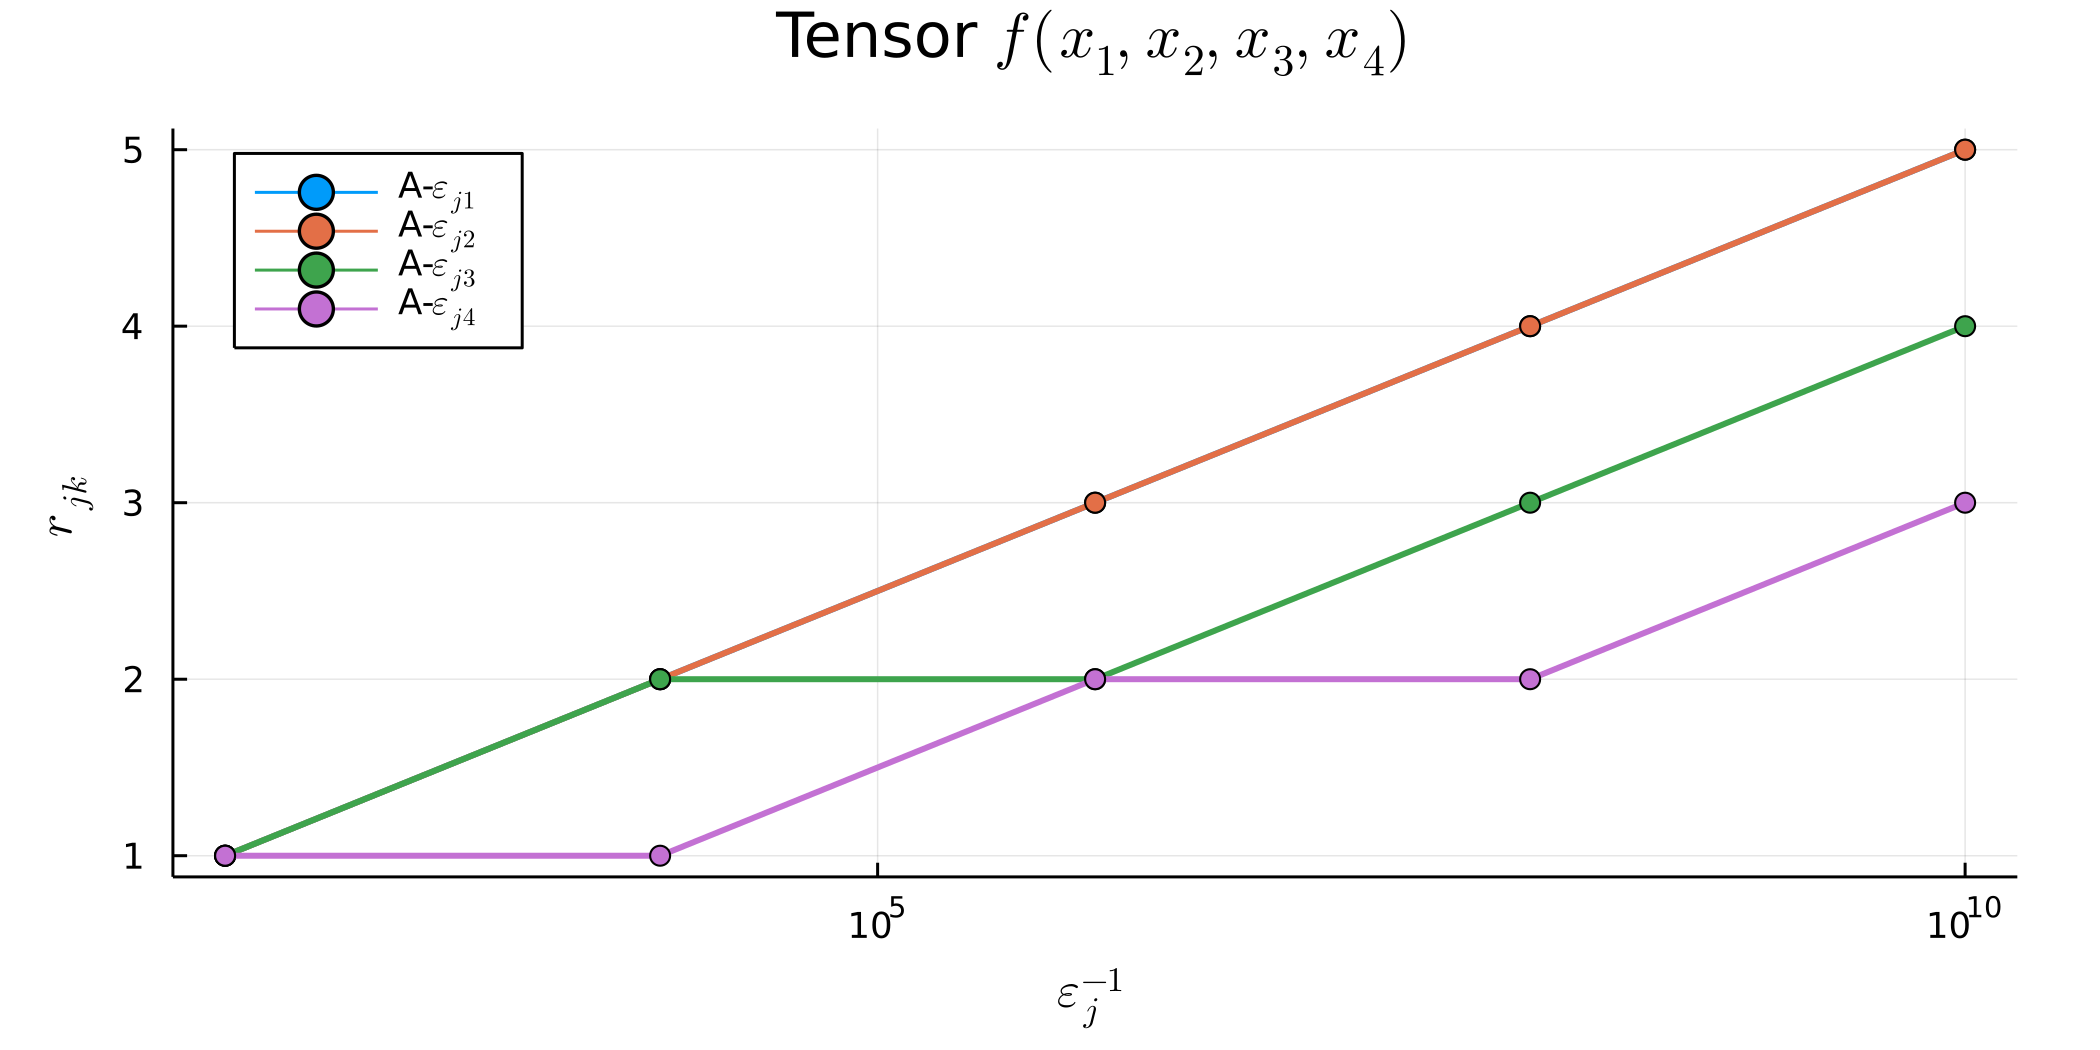
\includegraphics[width=0.49\textwidth]{./plots/hosvd-error-A.png}
    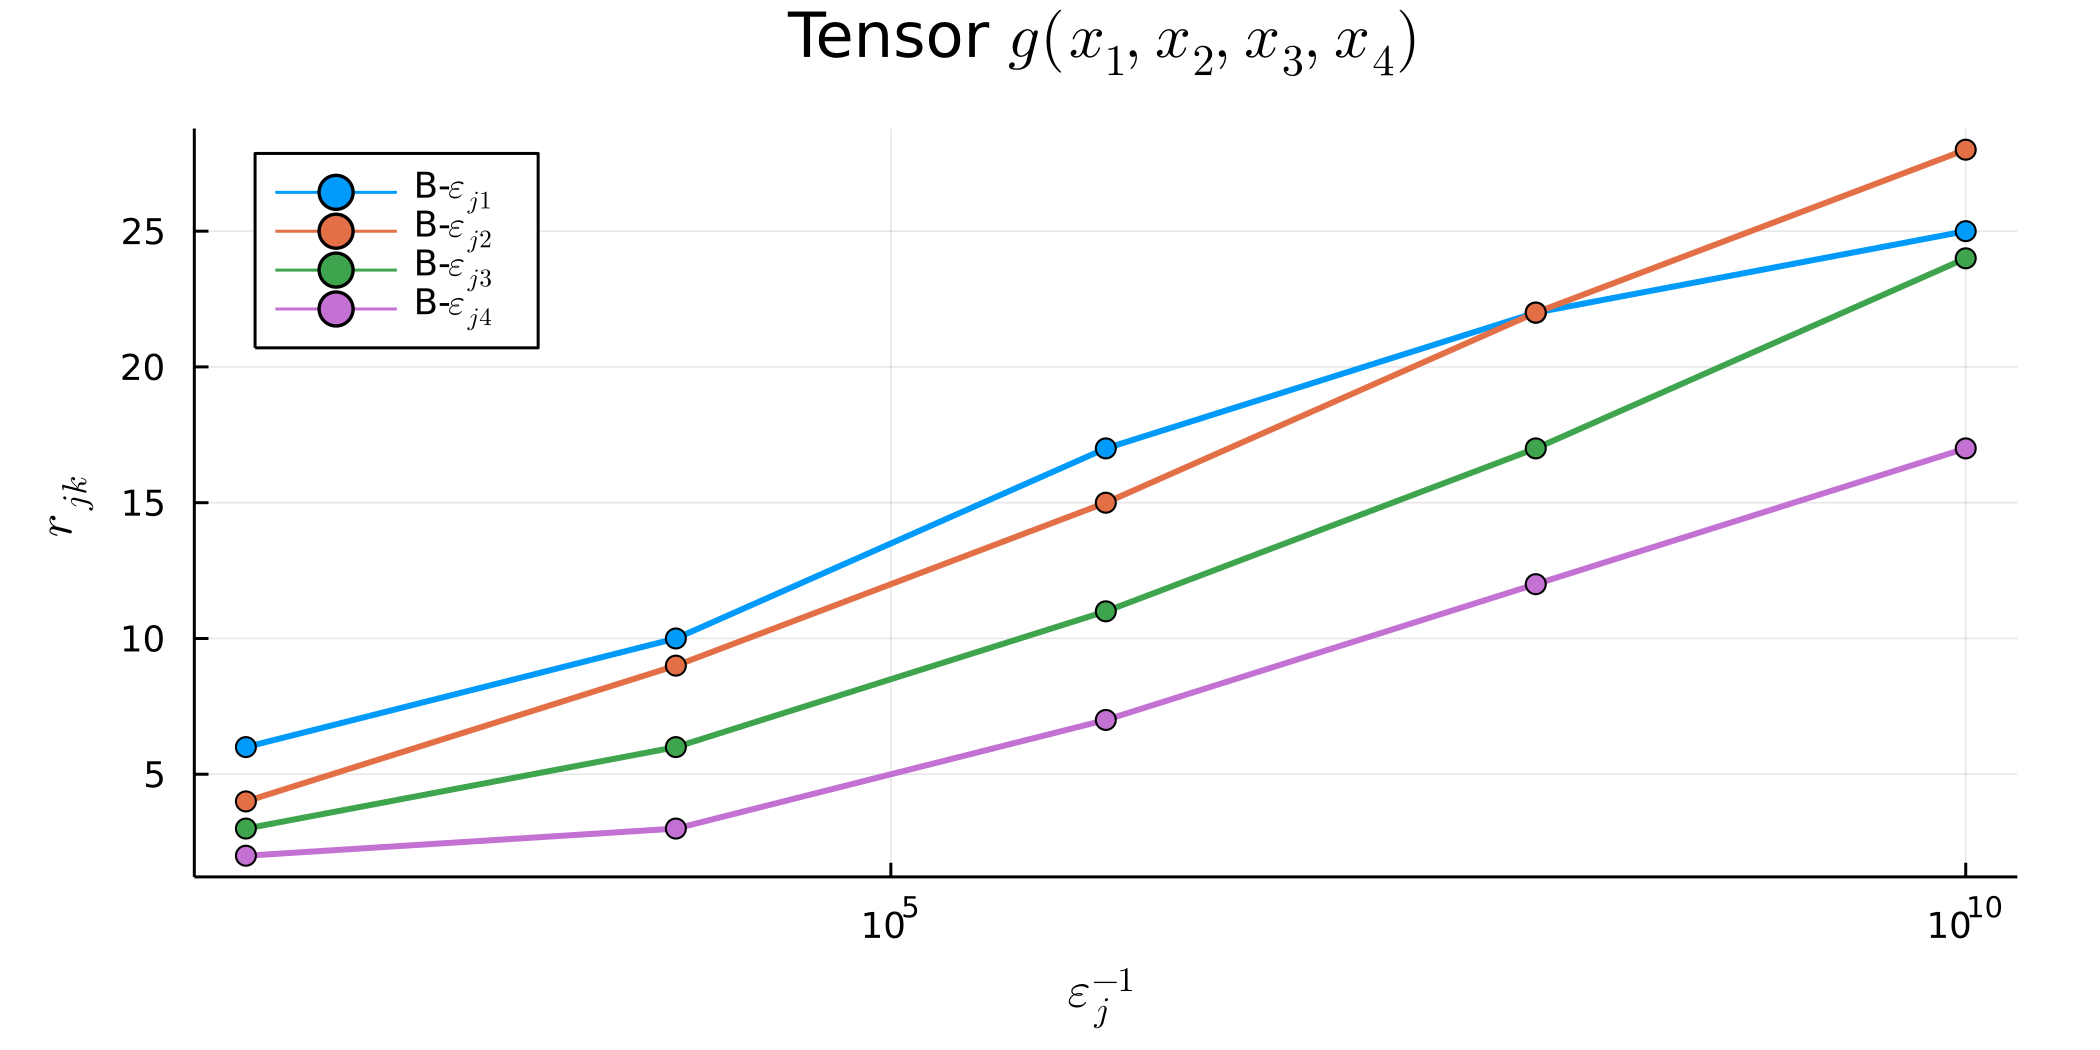
\includegraphics[width=0.49\textwidth]{./plots/hosvd-error-B.png}
    \caption{Dependence of the approximated ranks $r_{jk}$ on $j =
    \log_{10}\eps^{-j}$}
\end{figure}

For every $j$ we use our implementation of the HOSVD algorithm to compute the
Tucker approximation of $C$ for the ranks $r_{jk}$ for $k = 1, \cdots ,d$ and
the number of total entries $N_j$ produced by the output decomposition. In
the code \cite{code} it is checked during run-time that the error produced by
the HOSVD algorithm does not exceed $\|\eps_{jk}\|_F$ and agrees wit the
error analysis.

For $j = 12$ we plot the ratio of the singular values produced by the HOSVD
algorithm and during the SVD approximation of the $k-th$ Tucker unfolding
matrix
\begin{figure}[H]
    \centering
    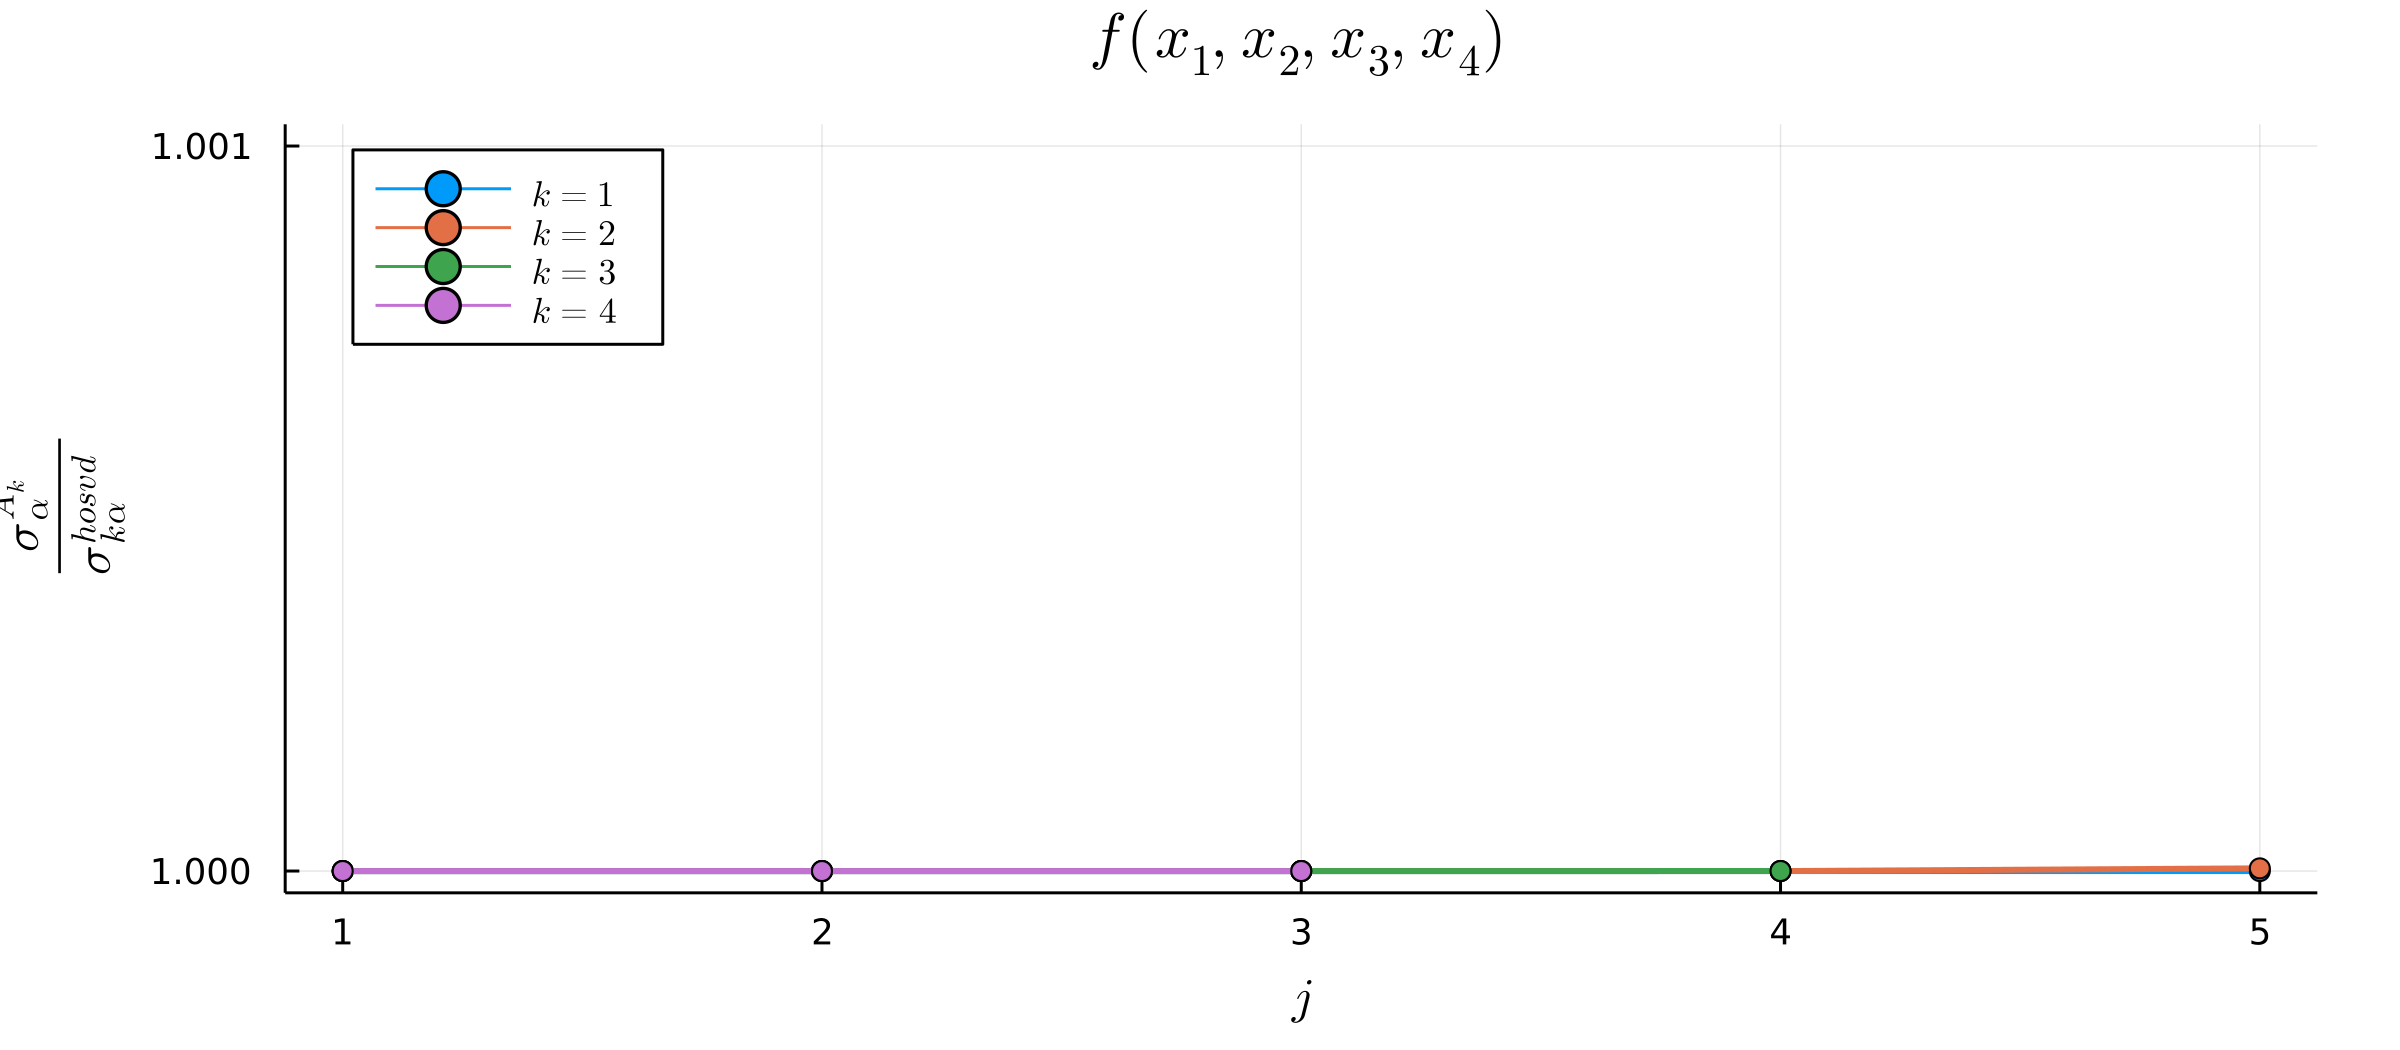
\includegraphics[width=0.49\textwidth]{./plots/hosvd-sigmaratio-a.png}
    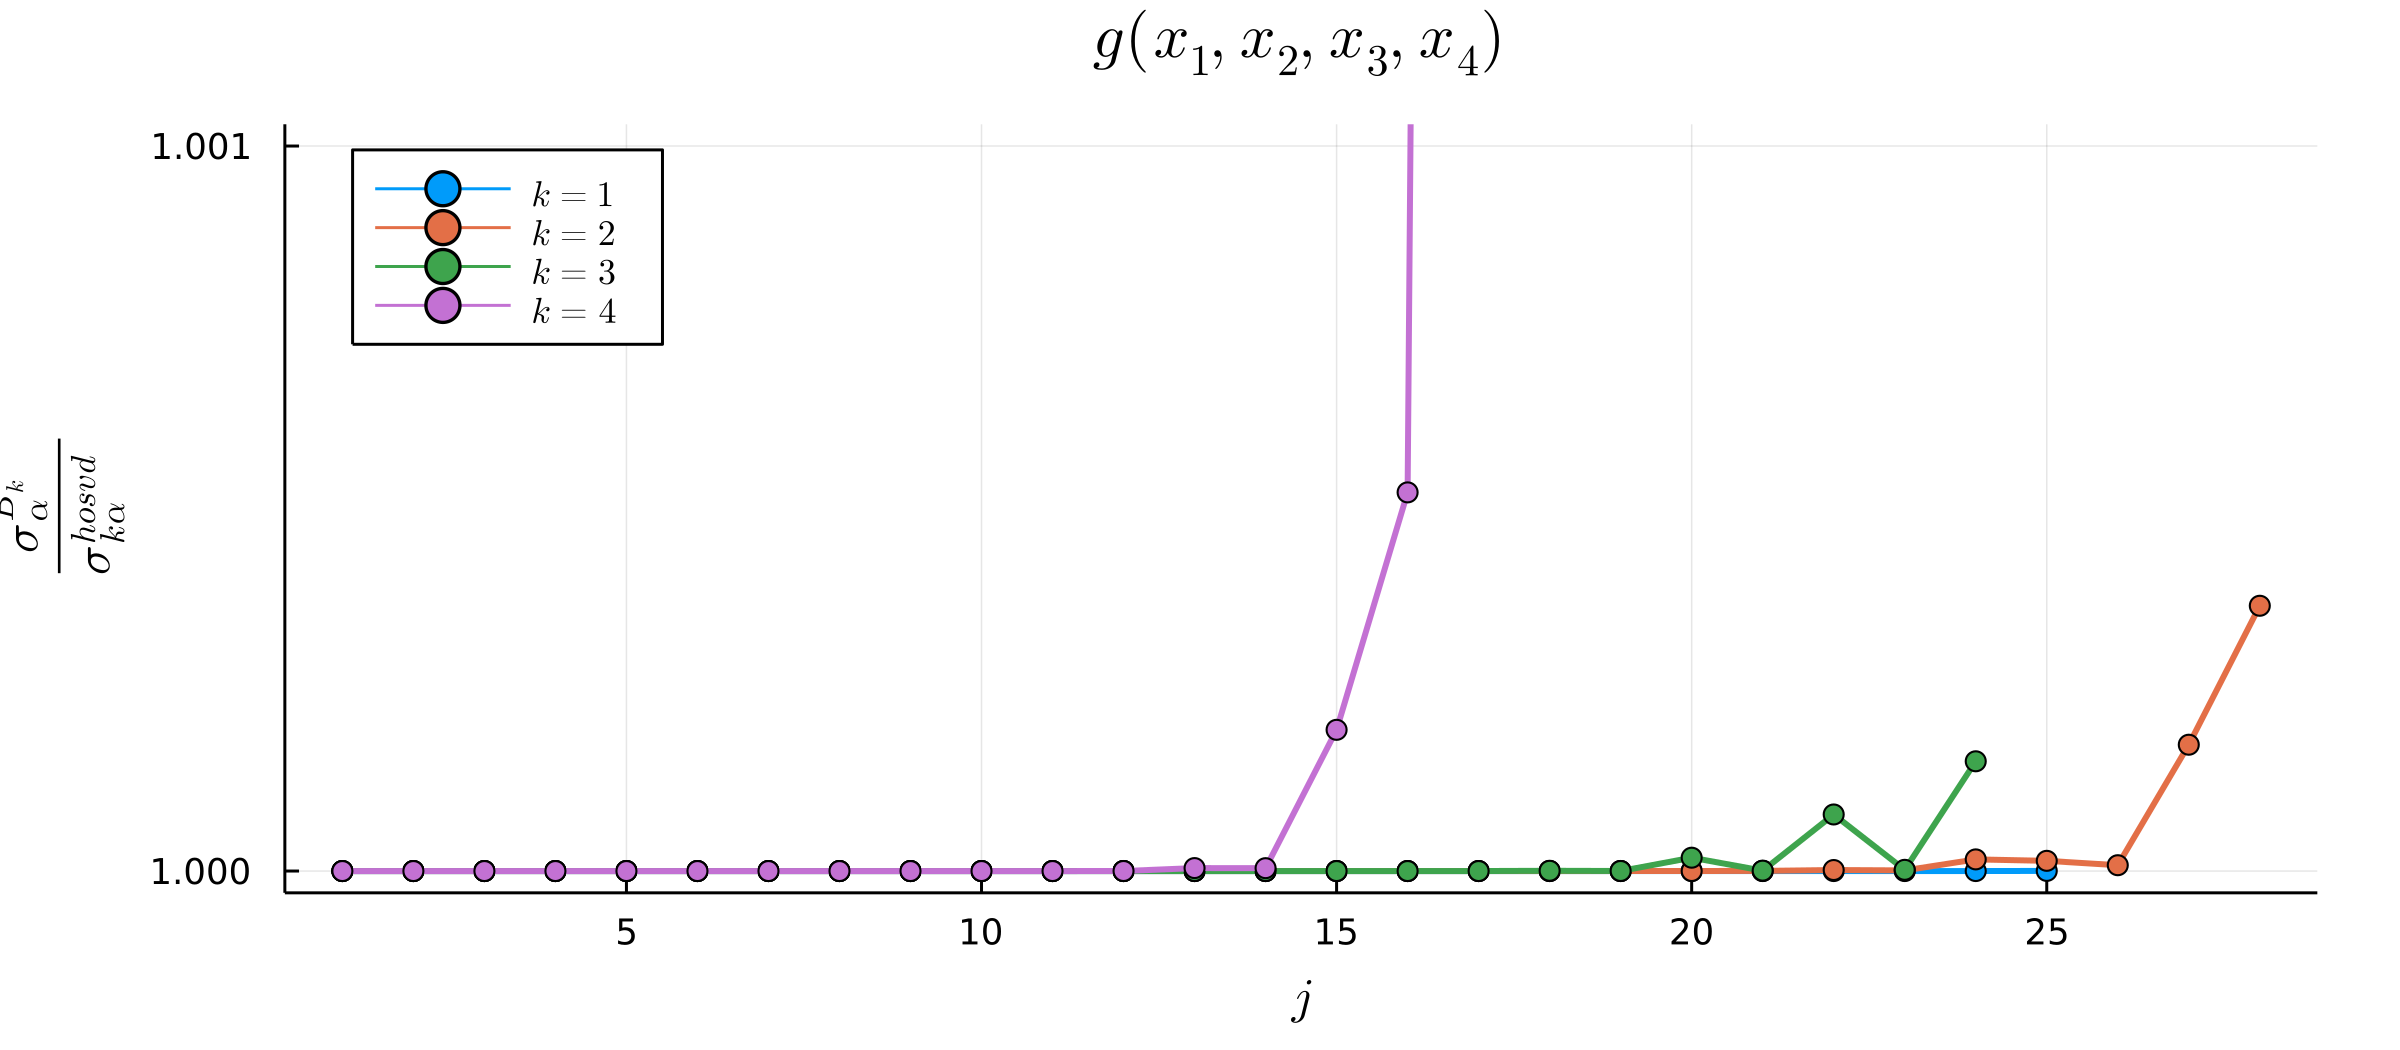
\includegraphics[width=0.49\textwidth]{./plots/hosvd-sigmaratio-b.png}
    \caption{Ratio of Singular values produced by the HOSVD and the $k-th$
    Tucker unfolding approximation of $C$.}
\end{figure}

\begin{figure}[H]
    \centering
    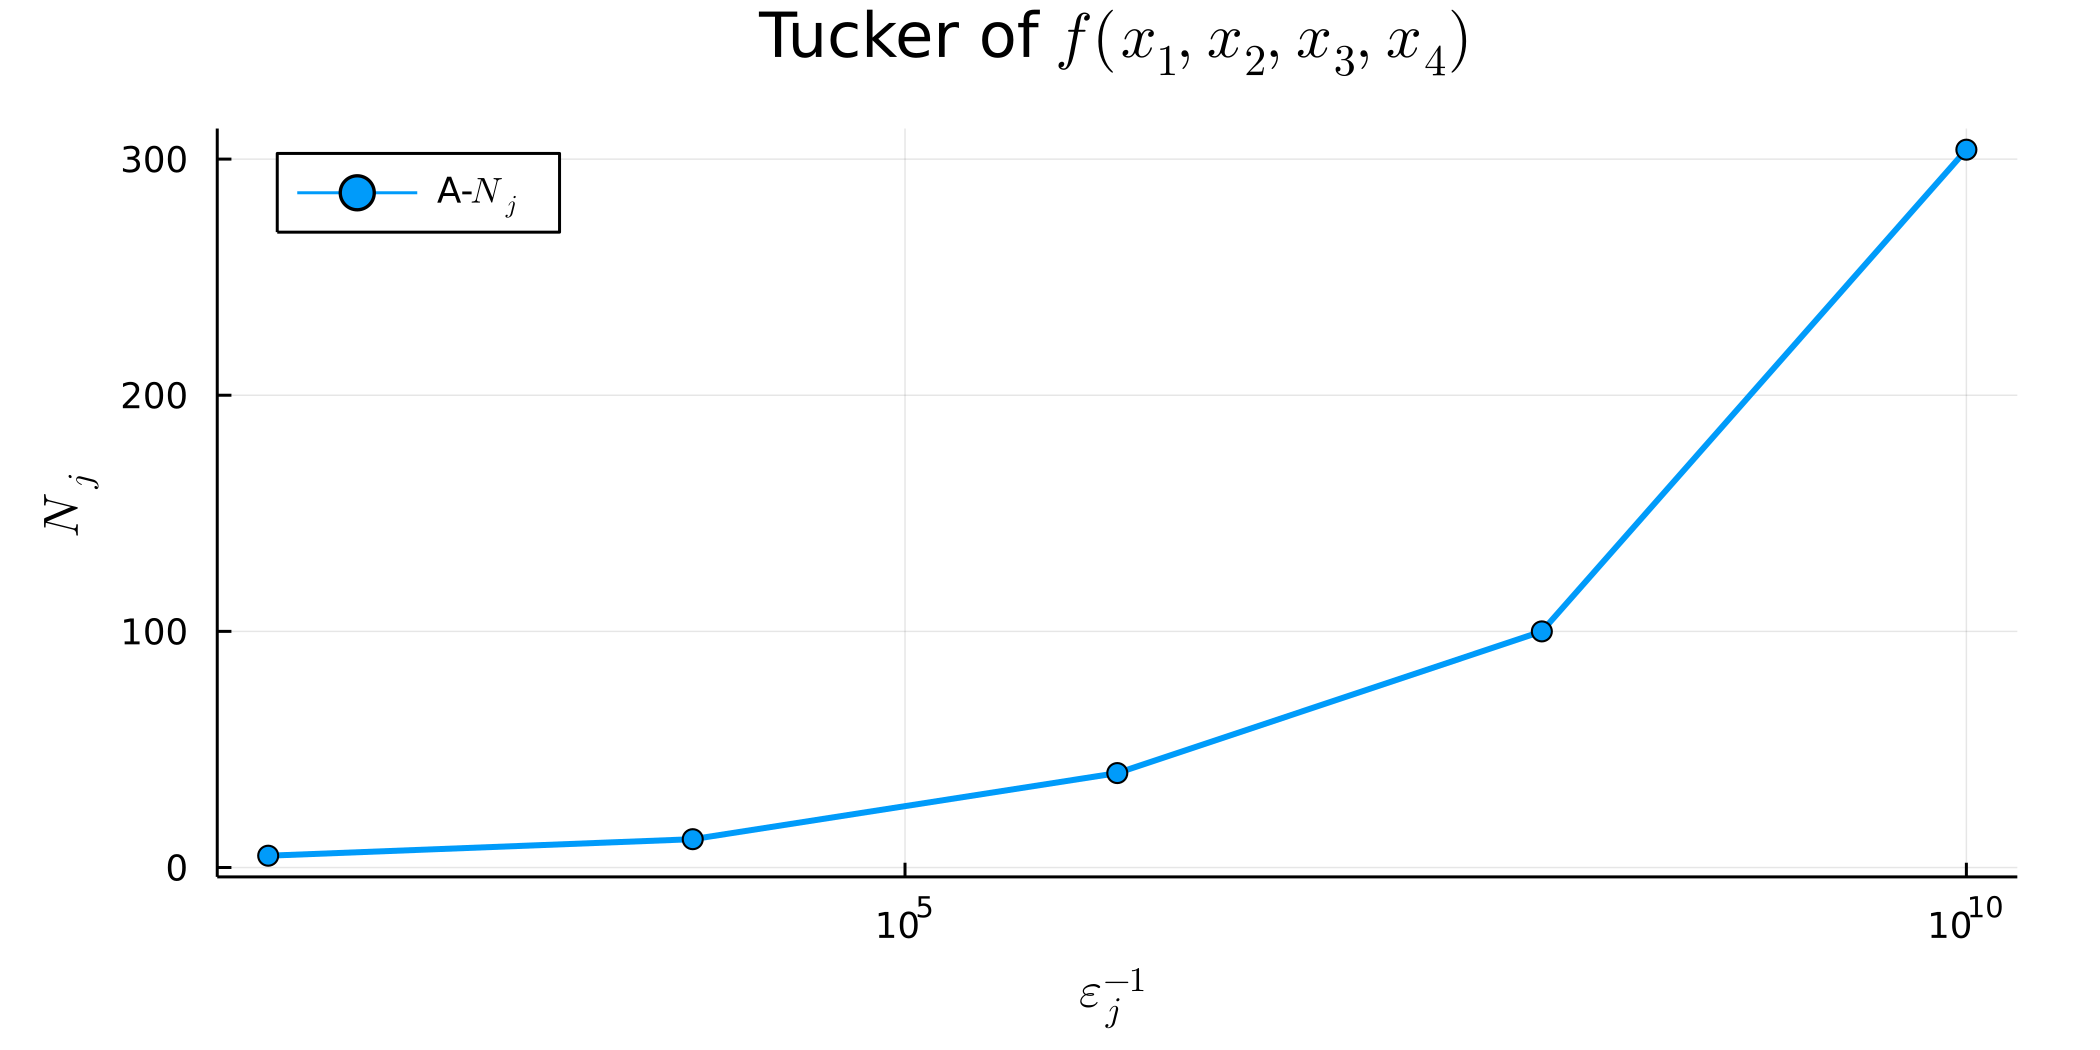
\includegraphics[width=0.49\textwidth]{./plots/hosvd-Nj-a.png}
    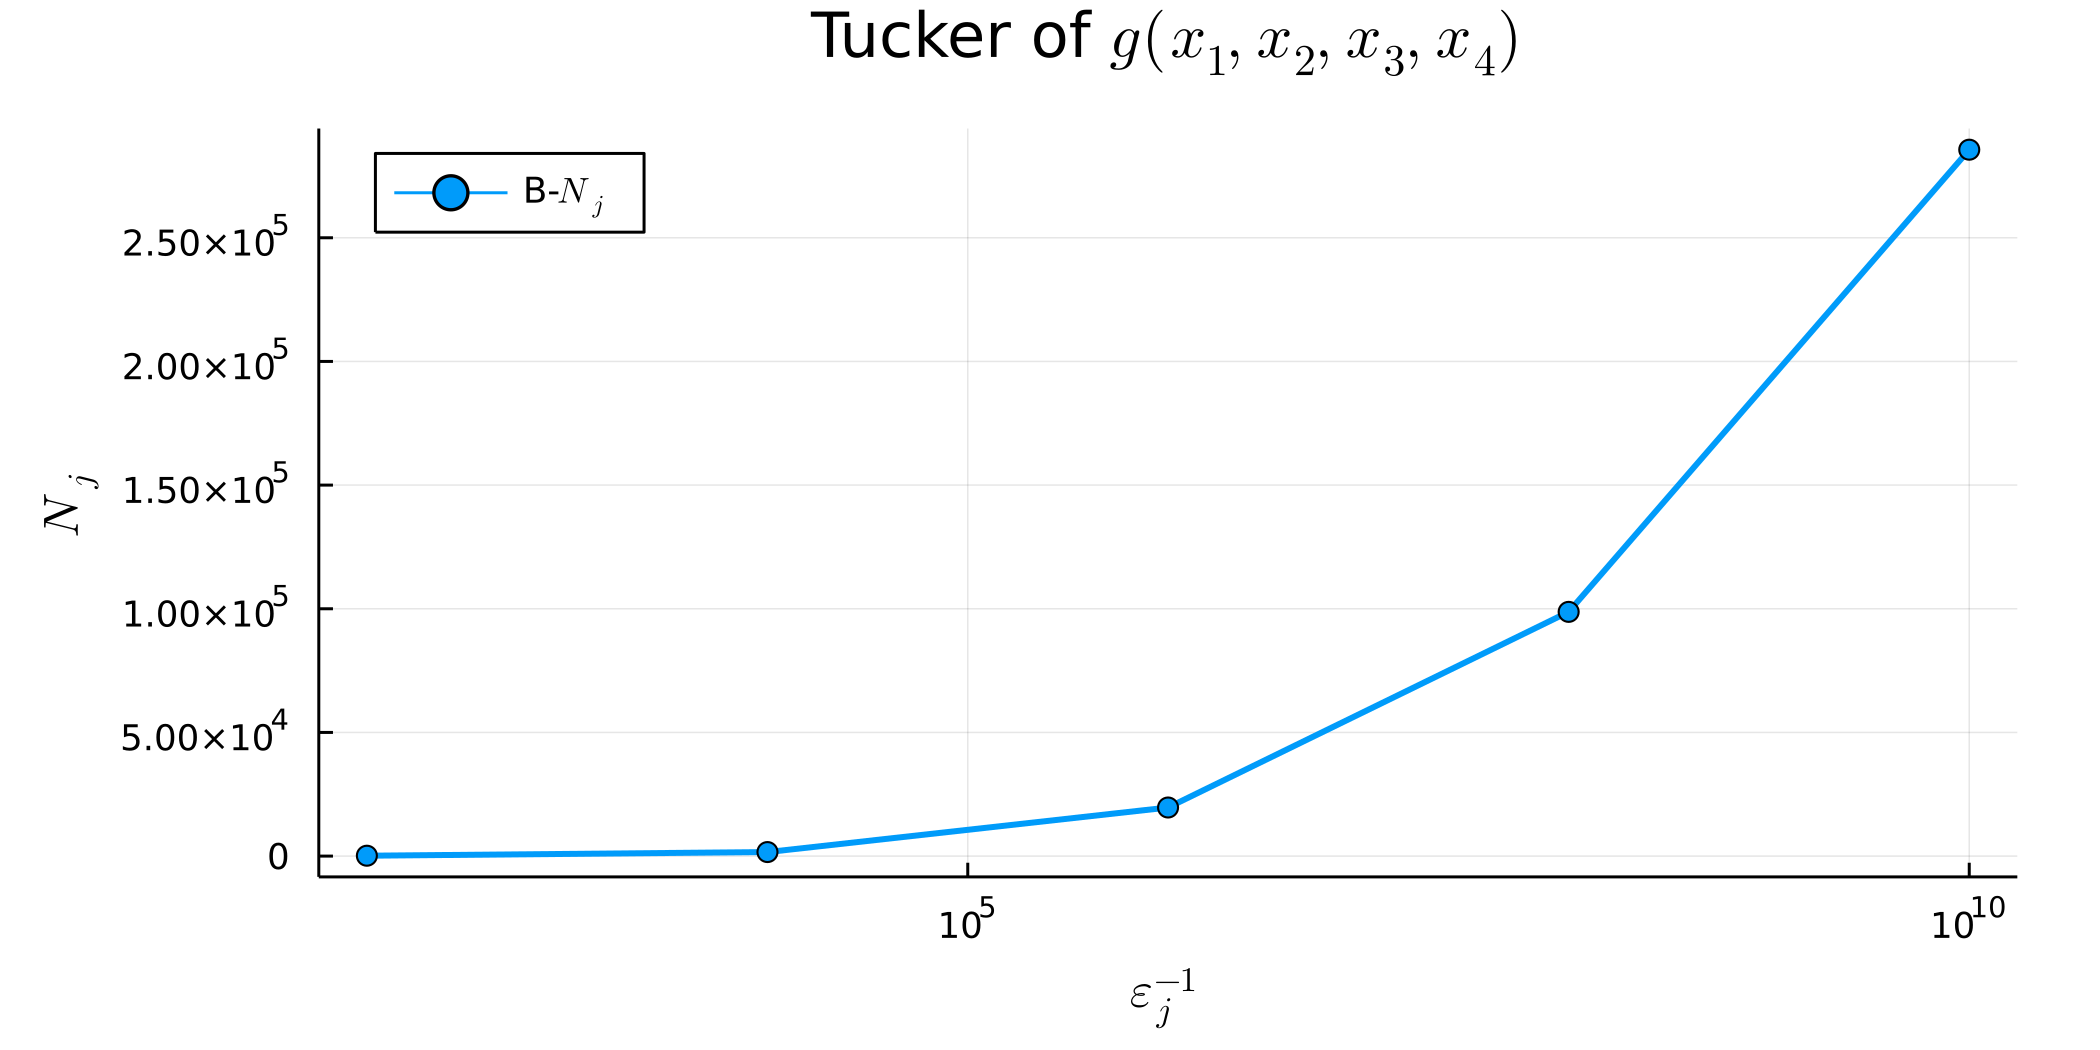
\includegraphics[width=0.49\textwidth]{./plots/hosvd-Nj-b.png}
    \caption{Number of parameters $N_j$ produced by the HOSVD for $C$}
\end{figure}


\subsection{TT-SVD for MPS-TT}
The TT-MPS (Tensor Train or Matrix Product States decomposition) for a given
tensor $A \in \mathbb{R}^{n_1 \times \cdots \times n_d}$ with ranks $r_1,
\dots, r_{d-1} \in \mathbb{N}$ is the following
\begin{align}
    A_{i_1,\dots, i_d} =
    \sum_{\alpha_1=1}^{r_1}\cdots\sum_{\alpha_{d-1}=1}^{r_{d-1}}U_1(\alpha_0,i_1,
    \alpha_1) \cdots U_d(\alpha_{d-1}, i_d, \alpha_d)
\end{align}
for $\alpha_0 = \alpha_d = 1$, $i_k \in \{1, \dots, n_k\}$. The
decomposition factors are given by
\begin{align}
    V_k(i_k) &\in \mathbb{R}^{r_{k-1}\cdot n_k \times r_k}, \\
    (V_k(i_k))_{\alpha_{k-1}, \alpha_k} &= U_k (\alpha_{k-1}, i_k, \alpha_k),
\end{align}
where $i_k$ is called the mode index.

The TT-SVD algorithm for $A$ as above is the following
\begin{algorithm}[H]
  \caption{TT-SVD algorithm}\label{alg: ttsvd}
\begin{algorithmic}
    \State $\hat{S}_0 \gets A$
    \State $A_0 \gets A$
    \State $r_0 \gets 1$
    \State $r_d \gets 1$
    \For{$k = 1, \dots, d-1$}
        \State $(B_k)_{\alpha_{k-1}\cdot i_k, i_{k+1} \cdots i_d} \gets
                (\hat{S}_{k-1})_{\alpha_{k-1}, i_k, i_{k+1}, \dots, i_d}$
                \Comment{reshape}

        \State $\hat{B}_k \gets \hat{U}_k \hat{\Sigma}_k \hat{V}_k^*$
        \Comment{rank $r_k$ T-SVD for $B_k$}

        \State $(\hat{C}_k)_{\alpha_{k-1},i_k,\alpha_k} \gets
        (\hat{U}_k)_{\alpha_{k-1}i_k, \alpha_k}$ \Comment{reshape}

        \State $(\hat{S}_k)_{\alpha_k, i_k, \dots, i_d} \gets
        (\hat{\Sigma}_k\hat{V}_k)_{\alpha_k, i_{k+1} \dots i_d}$
        \Comment{reshape}

        \State \text{save} $\frac{\| A - \hat{A}_k\|_F}{\|A\|_F}$
        \State \text{save} $\hat{C}_k$
        \State \text{save} $\hat{\Sigma}_k$
    \EndFor
\end{algorithmic}
\end{algorithm}
\subsection{Testing the TT-SVD}
For the case $d=4$ we construct a quasirandom Tucker decomposition by drawing
the entries for $C_k \in \mathbb{R}^{r_{k-1} \cdot n_k \times r_k}$  uniformly
on $[-1, 1]$. The output of the errors in the $k-th$ steps is in the figure
bellow
\begin{figure}[H]
    \centering
    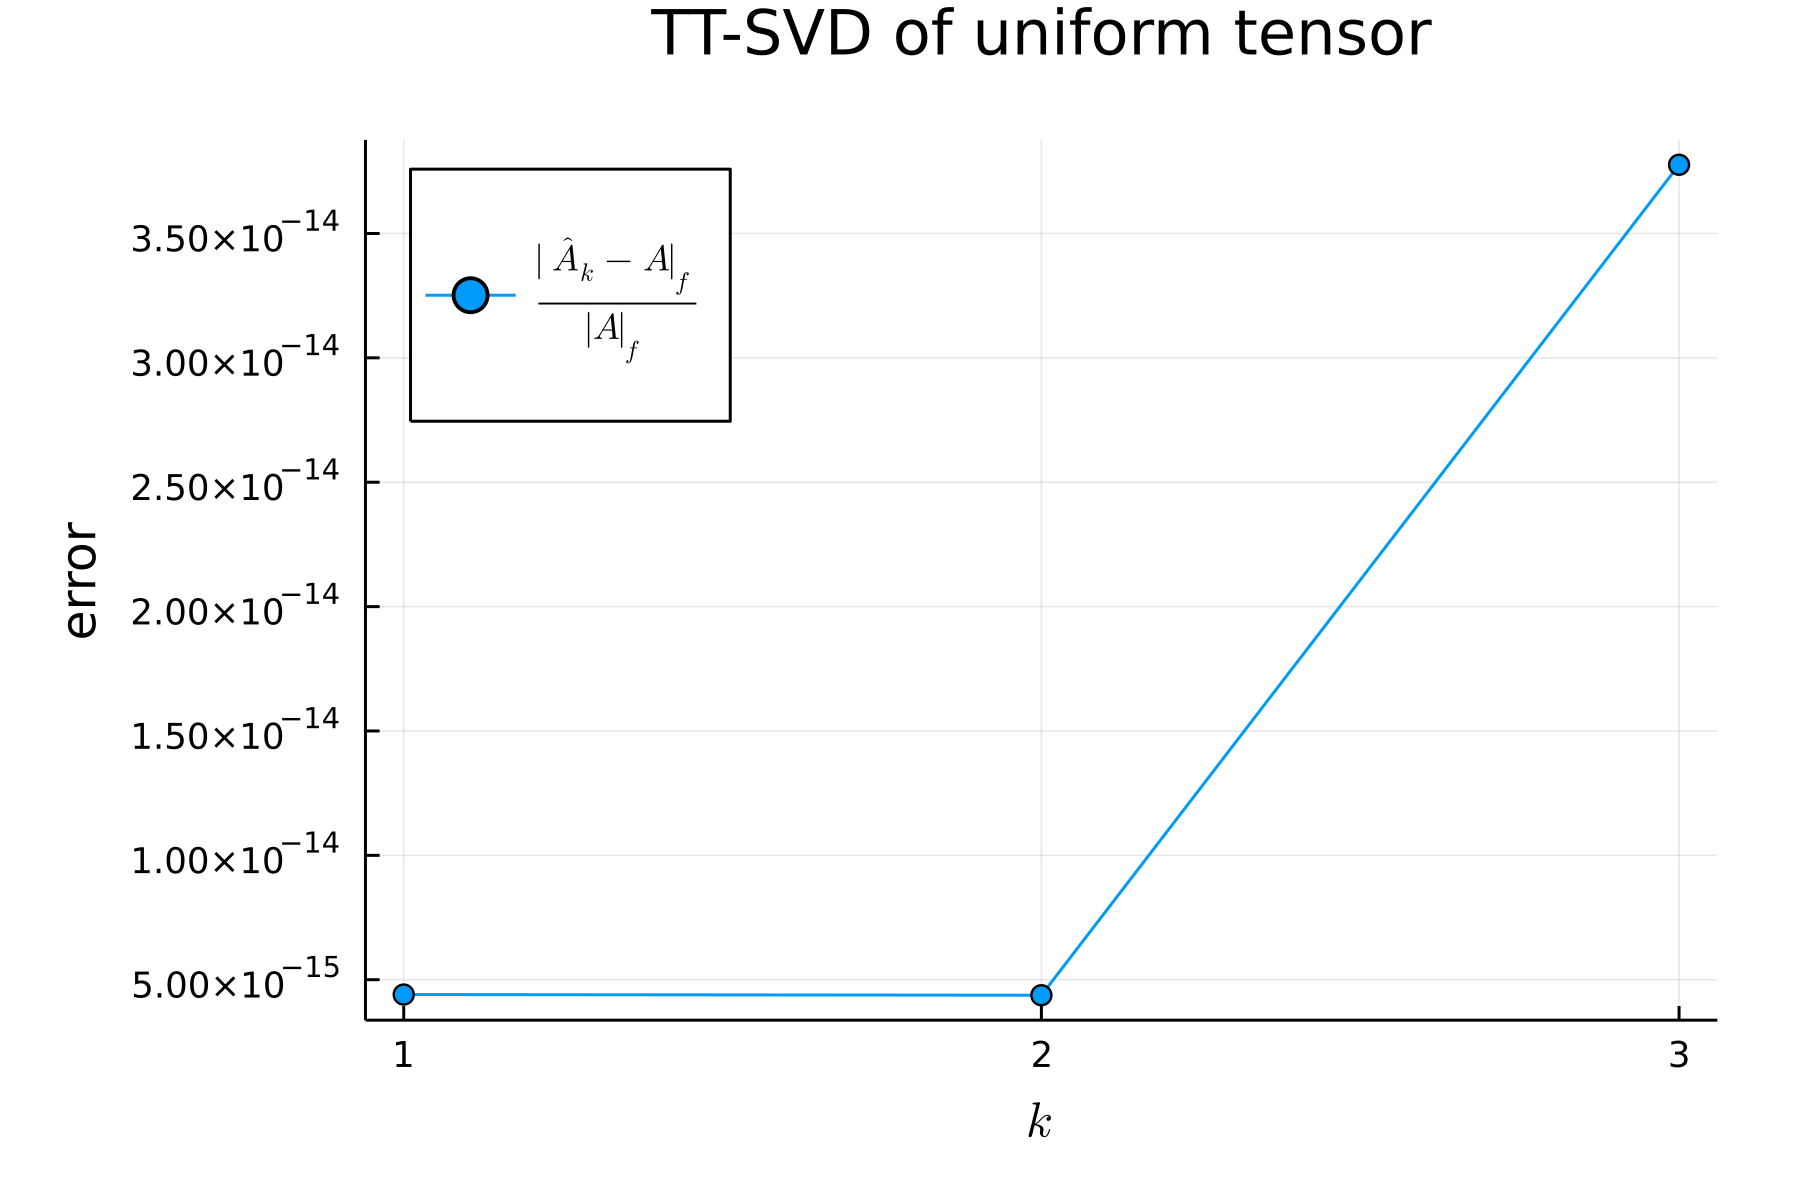
\includegraphics[width=\textwidth]{"./plots/ttsvd-uniform-error.png"}
    \caption{TT-MPS error on the $k-th$ step of a quasirandom Tensor in the
    TT-SVD algorithm}
\end{figure}
\subsection{TT-MPS of function-related tensors}
In this section we repeat everything we did in section \ref{sec: repeat},
replacing the HOSVD algorithm for the Tucker approximation with the TT-SVD
algorithm for the TT-MPS approximation

\begin{figure}[H]
    \centering
    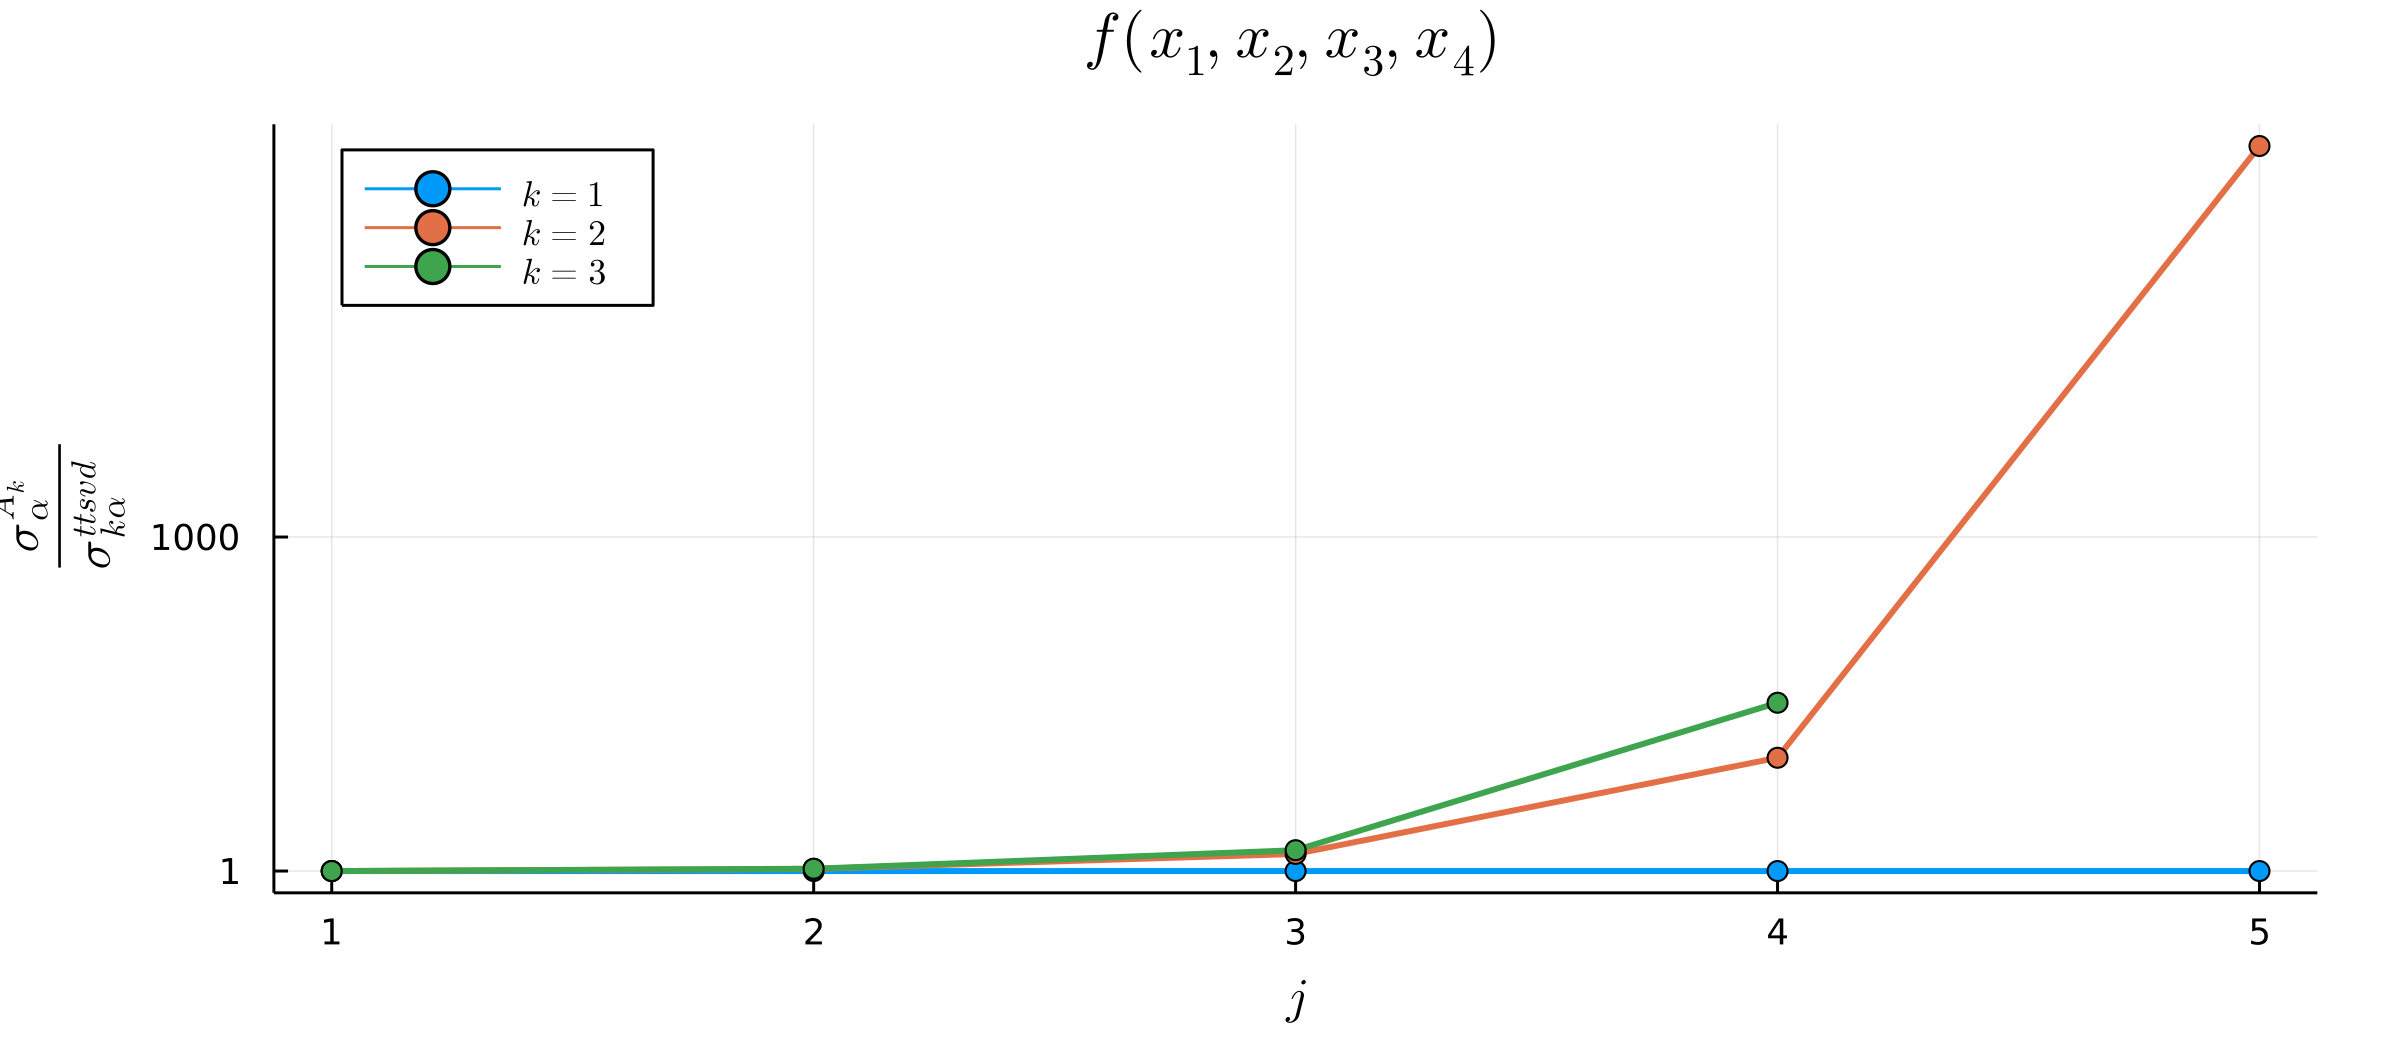
\includegraphics[width=0.49\textwidth]{./plots/ttsvd-sigmaratio-a.png}
    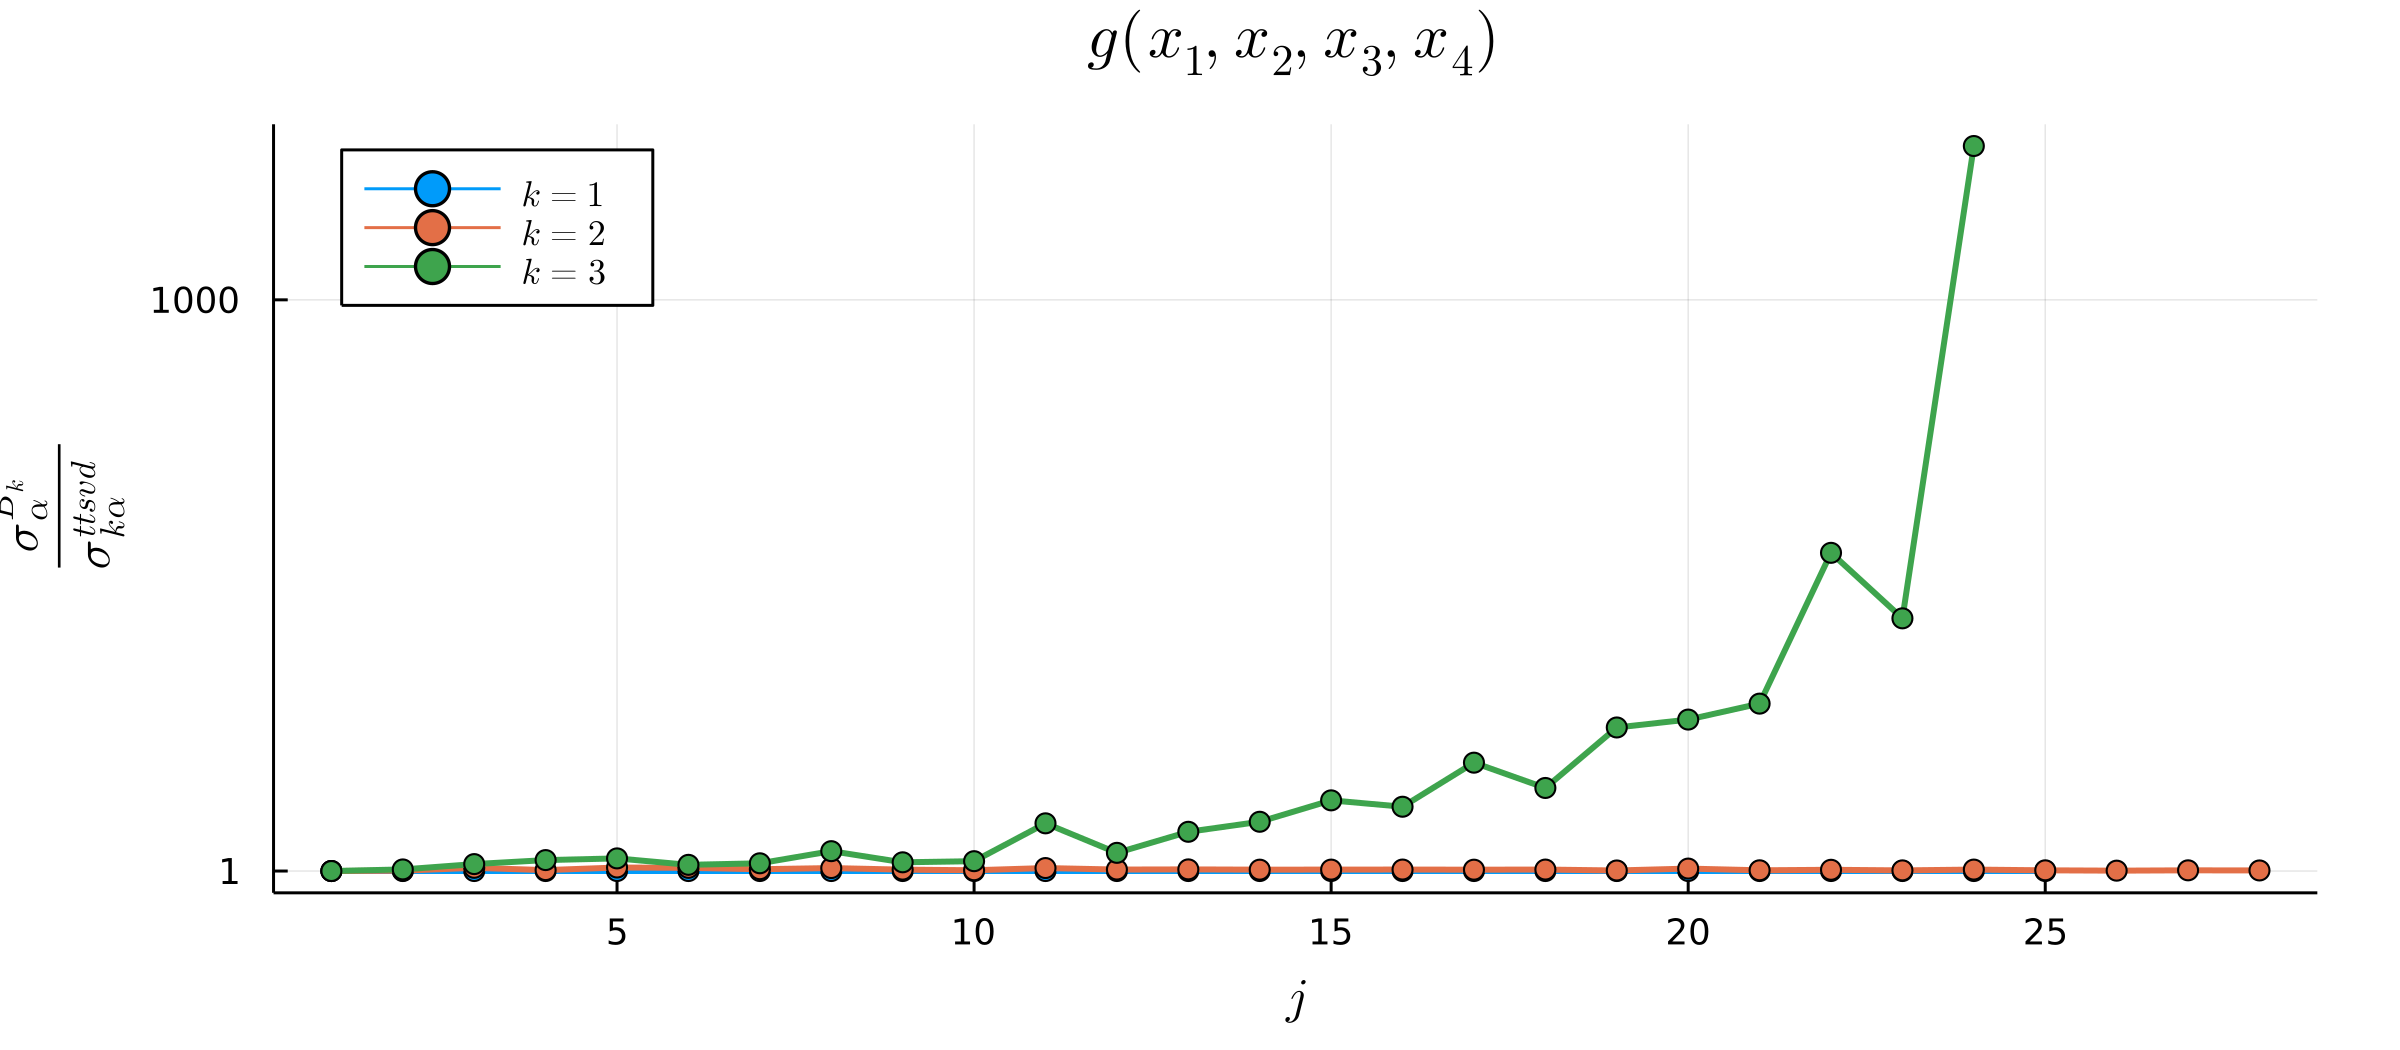
\includegraphics[width=0.49\textwidth]{./plots/ttsvd-sigmaratio-b.png}
    \caption{Ratio of Singular values produced by the TT-SVD and the $k-th$
    Tucker unfolding approximation of $C$.}
\end{figure}

\begin{figure}[H]
    \centering
    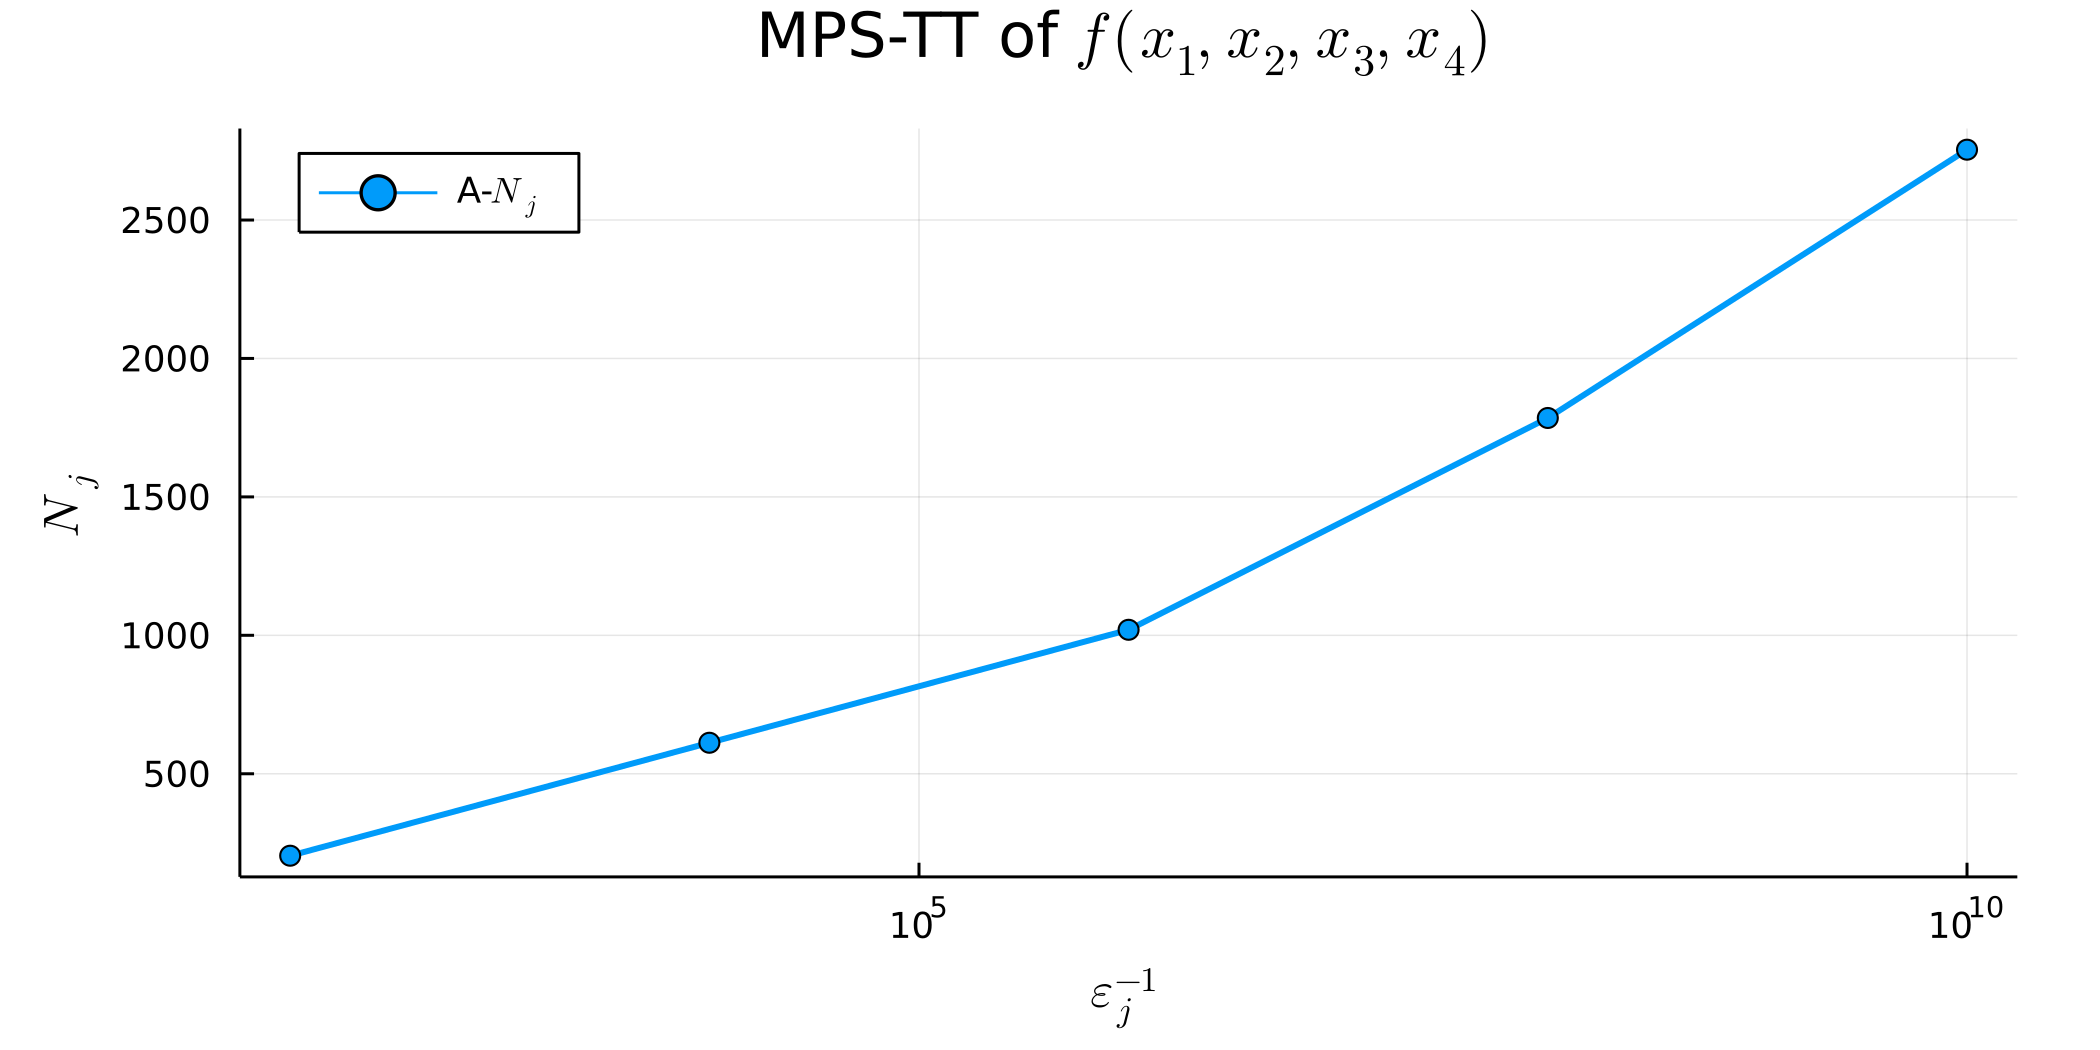
\includegraphics[width=0.49\textwidth]{./plots/ttsvd-Nj-a.png}
    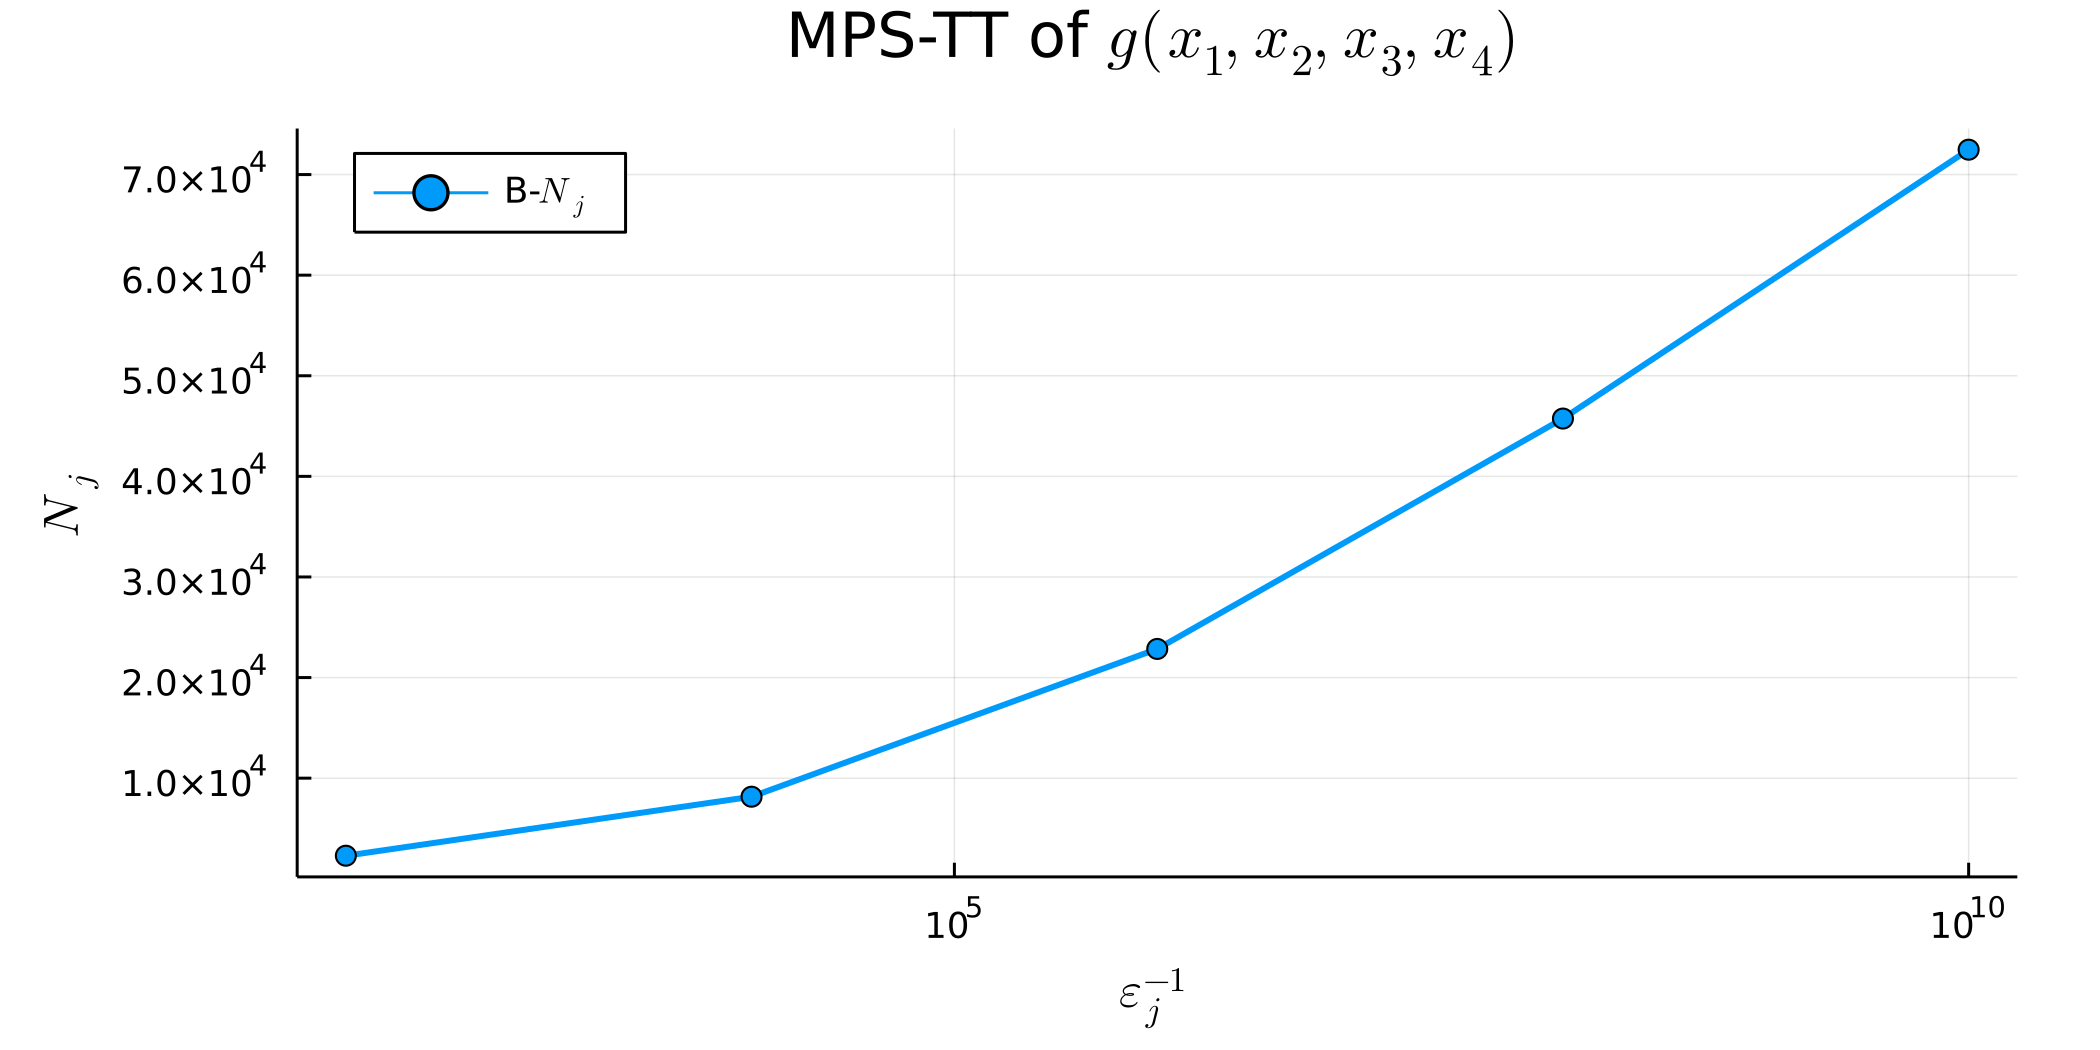
\includegraphics[width=0.49\textwidth]{./plots/ttsvd-Nj-b.png}
    \caption{Number of parameters $N_j$ produced by the TT-SVD for $C$}
\end{figure}


\nocite{code}
\printbibliography
\end{document}
